%Copyright 2014 Jean-Philippe Eisenbarth
%This program is free software: you can 
%redistribute it and/or modify it under the terms of the GNU General Public 
%License as published by the Free Software Foundation, either version 3 of the 
%License, or (at your option) any later version.
%This program is distributed in the hope that it will be useful,but WITHOUT ANY 
%WARRANTY; without even the implied warranty of MERCHANTABILITY or FITNESS FOR A 
%PARTICULAR PURPOSE. See the GNU General Public License for more details.
%You should have received a copy of the GNU General Public License along with 
%this program.  If not, see <http://www.gnu.org/licenses/>.

%Based on the code of Yiannis Lazarides
%http://tex.stackexchange.com/questions/42602/software-requirements-specification-with-latex
%http://tex.stackexchange.com/users/963/yiannis-lazarides
%Also based on the template of Karl E. Wiegers
%http://www.se.rit.edu/~emad/teaching/slides/srs_template_sep14.pdf
%http://karlwiegers.com
\documentclass[16pt]{scrreprt}
\usepackage{listings}
\usepackage{float}
\usepackage{setspace}
\usepackage{url}
\usepackage{longtable}
\usepackage{booktabs}
\usepackage{underscore}
\usepackage{graphicx, subfig}
\usepackage[bookmarks=true]{hyperref}
\usepackage[utf8]{inputenc}
\usepackage[english]{babel}

\hypersetup{
    bookmarks=false,    % show bookmarks bar?
    pdftitle={Software Requirement Specification},    % title
    pdfauthor={Jean-Philippe Eisenbarth},                     % author
    pdfsubject={TeX and LaTeX},                        % subject of the document
    pdfkeywords={TeX, LaTeX, graphics, images}, % list of keywords
    colorlinks=true,       % false: boxed links; true: colored links
    linkcolor=blue,       % color of internal links
    citecolor=black,       % color of links to bibliography
    filecolor=black,        % color of file links
    urlcolor=purple,        % color of external links
    linktoc=page            % only page is linked
}%
\def\myversion{1.0 }
\date{}
%\title
\usepackage{hyperref}
\DeclareOldFontCommand{\bf}{\normalfont\bfseries}{\mathbf}
\begin{document}

\begin{flushright}
    \rule{16cm}{5pt}\vskip1cm
    \begin{bfseries}
        \LARGE{SOFTWARE REQUIREMENTS\\ SPECIFICATION}\\
        \vspace{0.8cm}
        for\\
        \vspace{0.8cm}
        iSport\\
        \begin{figure}[H]
		\flushright
  		
\includegraphics[width=.2\textwidth]{figures/logo.png}
		\end{figure}
        \vspace{0.8cm}
        \normalsize{Version \myversion approved}\\
        \vspace{1.0cm}
        Prepared by\vspace{0.5cm} \\ 
        \normalsize{1650940 Jiang Xiaohu\\1650932 Xu Jingnan\\1651058 Wang Yicheng}
        \\
        \vspace{1.1cm}
        \normalsize{School of Software Engineering\\ Tongji University}\\
        \vspace{1.0cm}
        \today\\
    \end{bfseries}
\end{flushright}

\tableofcontents


\chapter*{Revision History}

\begin{center}
    \begin{tabular}{|p{5cm}|p{3cm}|p{7cm}|p{2cm}|}
        \hline
	    Name & Date & Reason For Changes & Version\\
        \hline
	    Jiang Xiaohu & 2019.11.1 & Finish Introduction Part  & v1.0\\
        \hline
	    Wang Yicheng & 2019.11.2 & Finish Overview Part & v1.1\\
        \hline
        Xu Jingnan & 2019.11.3 & Finish External Requirements Part & v1.2\\
        \hline
        Xu Jingnan, Jiang Xiaohu, Wang Yicheng & 2019.11.4 & Finish Sequence Diagrams for Function Modeling Part& v1.3\\
        \hline
        Xu Jingnan & 2019.11.5 & Finish Function Modeling Part & v1.4\\
        \hline
        Jiang Xiaohu & 2019.11.6 & Finish Data Modeling Part  & v1.5\\
        \hline
    \end{tabular}
\end{center}

\chapter{Introduction}

\section{SRS Purpose}
The purpose of this document is to present a detailed description of iSport. It will explain the purpose and features of iSport, the interfaces of the iSport, the functional and nonfunctional requirements of iSport, what iSport will do, and the constraints under which it must operate and how the system will react to external stimuli. This document is intended for both the stakeholders and the developers of the system and will be proposed to the clients for its approval.
%This SRS (Software Requirements Specification) document aims to identify the product--iSport whose software requirements are specified in this 
%document, including the revision or release number. And the scope of iSport is covered by this SRS, too, particularly if this SRS describes only 
%part of the system or a single subsystem.$>$

\section{Product Scope}
This software system will be a web based system for sports fans, professional athletes, and patients who are under recovering training. \\
\\
This system will be designed to maximize the exercising efficiency by providing tools to assist in checking and correcting user's wrong postures and recommending training courses customized for users, which would otherwise have to be expensive, time-consuming and labor intensive. By maximizing the user’s training efficiency and convenience the system will meet the needs of sports fans, athletes and injured patients while remaining easy to understand and use.\\
\\
More specifically, this system is designed to allow a user to imitate the standard exercising postures while observe and correct their mistakes simultaneously with the help of a website. \\
\\
The software will collect some professional courses in the database, including static and dynamic trainings which means doing exercise according to a set of images or a video and iSport will recommend suitable trainings for users on the basis of their training performance. Courses are classified into exercising courses and recovering courses, aiming to help athletes and patients respectively.\\
\\
Both visual and audio notification are used in every course of the system to provide eye-catching, user-friendly and clear instructions; the feedback of one's training is proposed once the training is over and the report can be browsed in the report page.\\
\\
The selection and deletion of one user's favorable course is supported in personal information webpage and one can comment training he/she has taken on comment webpage to provide suggestions to other users.\\
\\
 The personal information registering, changes is allowed via the application options. The system also contains a relational database containing a list of users, training images and videos.
 
\section{Intended Audience}
This Software Requirements document is intended for:
\begin{itemize}
	\item Developers who can review project’s capabilities and more easily understand where their efforts should be targeted to improve or add more features to it (design and code the application – it sets the guidelines for future development).
	\item Project testers can use this document as a base for their testing strategy as some bugs are easier to find using a requirements document. This way testing becomes more methodically organized.
   \item End users of this application who wish to read about what this project can do.
   \item Clients who delegate the software development to our team, and can check if their requirements are perfectly understood by the developers and whether the functional and nonfunctional requirements are entirely meet. And they can modify some requirements according to this document in later stage. 
   \item Project managers who translate the clients' requirement to the programmers and supervise them to implement the requirements mentioned in the documents and if the clients modify the requirements, the project managers have to negotiate the changes with the clients and modify the document.
   \item Marketing staff who are responsible to sale and prompt the software should be clear about what iSport can do, what iSport's advantages are, what iSport's competitive power is.
   \item Service staff who are responsible to solve the customer's problems, they have to know what iSport can do and feedback the technical problems to developers.
   \item Document writers who are responsible for writing the rest documents in later development stages should follow the requirements specified in this SRS.
\end{itemize}
The rest part of this SRS document contains the overall description of iSport, and iSport's specific, nonfunctional and other requirements which are shown in chapter\ref{Overall Description}, chapter\ref{Specific Requirements}, chapter\ref{Other Nonfunctional Requirements} and chapter\ref{Other Requirements} respectively.
We suggest the readers begin with the overview sections and proceeding through the sections that are most pertinent to them:
\begin{itemize} 
	\item Developers and project testers are recommended to focus on specific and nonfunctional requirements part because theses parts will lead them to build qualified, safe and satisfying application and theses parts are all related to coding (construction and verification stage).
	\item Clients, project managers and document writers should focus on the entire document since they are responsible for all the requirements specified in this paper.
	\item Marketing staff have to focus on the functional part of iSport.
\end{itemize}


\section{Definitions, Acronyms, and Abbreviations}
\begin{longtable}{|p{1.9in}|p{4in}|c|}
xxxxx & xxxxxx  \kill
\caption{Definitions\label{simple}}\\ \hline
\multicolumn{3}{|c|}{\bf Definitions, Acronyms, and Abbreviations}\\ \hline
\endfirsthead
\caption[]{(continued)}\\ \hline
\multicolumn{3}{|c|}{\bf Definitions, Acronyms, and Abbreviations (continued)}\\
\hline
\endhead
\hline
\multicolumn{3}{|c|}{\bf Continued $\ldots$}\\
\hline
\endfoot
\hline
\multicolumn{3}{|c|}{\bf The End}\\
\hline
\endlastfoot
Term & Definitions  \\
\hline
User & Someone who interacts with iSport including sports fans, athletes and  injured patients who need recovery training.\\  \hline  
Sports fans & One of iSport's potential customers who love sports and want to get professional instructions when exercising. Some of them may can't afford the expense of personal coaching or don't have time to go to the gym. \\ \hline
Athletes & One of iSport's potential customers who want to get real-time exercising feedback to improve their performance or who want to get some relaxing training in their spare time to keep a good competitive state.\\  \hline
Injured Patients & One of iSport's potential customers who need recovering training after some treatments, e.g. surgeries. On the one hand, some of them may can't afford the doctor's expensive medical instructions for recovering training. on the other hand, there is no enough doctors or nurses who can instruct and supervise the patients' recovering exercising. But without professional instructions training can be useless or even leads to secondary trauma.\\  \hline
Admin/Administrator & System administrator who is given specific permission for managing and controlling the system, e.g. updating the user's information, uploading new training courses.\\ \hline
User Info & User's basic information including user's avatar, account name, tel-number and email address.\\ \hline
Courses & Training courses including normal exercising training and recovering training.\\ \hline
Exercise Courses & Training courses which serve the sports fans and athletes.\\ \hline
Recover Courses & Training courses which serve the injured patients.\\ \hline
Static Courses & Training courses which instruct the users photo by photo.\\ \hline
Dynamic Courses & Training courses which instruct the users according to a standard video.\\ \hline
Appraisal Subsystem & Remark the user's performance by using a grade from 0 -100\\ \hline
Comment Subsystem & User comment on the training courses they have taken to provide reference for other users.\\ 
\hline 
Recommendation Subsystem & A subsystem which will provide some courses for users according to their recent performance.\\ 
\hline
Exercise Tips & There will be sports tips in the webpage of iSport to prevent users from athletic injuries.\\ 
\hline 
Sport Report & A web page to feedback the user's exercising performance.\\ 
\hline 
Audio Notification & An audio notification will be shown when the user is doing exercise to encourage the user to hold on or notify the user to correct their postures.\\ 
\hline 
Visual Notification & A visual notification will be shown when the user is doing exercise, if the user's posture is standard, then the web-frame will turn green to suggest the user to hold on, otherwise the web-frame will be red.\\ 
\hline 
DataBase & A relational database containing a list of user info, training images and videos.\\ 
\hline 
Detection Subsystem & Subsystem to detect the user's postures and draw the user's skeleton. The main model of detection subsystem is PoseNet.\\ 
\hline 
Comparison Subsystem & Subsystem to compare the postures of the user and that of the standard. The subsystem aims to check if the user pass the posture.\\ 
\hline 
Correction Subsystem & Subsystem to calculate where the postures' wrong part are, e.g. left-arm, right-leg, head.\\ 
\hline 
Clients & Group who delegate the development of iSport to the developers and will take charge of the later management of iSport.\\ \hline
Developers & Develop team including project managers, programmers, testers who are responsible for the development of iSport and its later mainteinance and updating.\\ 
\hline 
\end{longtable}

\section{Document Conventions}
This document follows MLA Format[1]. Bold-faced text has been used to emphasize sectionand sub-section headings. Highlighting is to point out the references of tables and figures. Underline is used in CRC's grammar analysis. And italicized text is used to label and recognize special characters or terminologies\\

\noindent The SRS paper is written by latex[6], the packages we used to format the document including \small{$longtable, graphicx, subfig, utf8-inputenc,hyperref$ }and so on.\\

\noindent And we modified the IEEE SRS latex template from Jean-Philippe Eisenbarth's github[7] according to the IEEE standard[2] mentioned in Frank F Tusi'book[3].\\

\noindent Finally, figures we use in the document is drawn by Staruml[8] and ProcessOn[9]

\section{References and Acknowledgements}
\subsubsection{Standard References}
The standards we have followed are as follows:\\

$[1]$ T. Russell, A. Brizee, E. Angeli, and R. Keck, “Mla formatting and style guide,” The Purdue OWL, 2010.\\

$[2]$ I. S. E. S. Committee et al., “Ieee recommended practice for software re- quirements specifications,” IEEE organization, 1998.\\


$[3]$ F. F. Tsui, O. Karam, and B. Bernal, Essentials of software engineering. Jones Bartlett Learning, 2016.\\

$[4]$ R. S. Pressman, Software engineering: a practitioner’s approach. Palgrave Macmillan, 2005.\\

$[5]$ P. Coad, E. Yourdon, and P. Coad, Object-oriented analysis. press Englewood Cliffs, NJ, 1991, vol. 2.
\subsubsection{Writing Tools References}
The writing tools we have used are as follows:\\

$[6]$L. Lamport, LATEX: a document preparation system: user’s guide and reference manual. Addison-wesley, 1994.\\

$[7]$ J.-P. Eisenbarth, “Srs latex template under ieee standard,” \\http://https://github.com/jpeisenbarth/SRS-Tex.\\

$[8]$ S. Wong, “Staruml tutorial,” Connexions Web site, Sep, 2007.\\

$[9]$ P. O. Team, “Process on tools,” https://www.processon.com/support.

\chapter{Overall Description}
\label{Overall Description}

\section{Product Perspective}

ISport is a web system developed by isport team, aimming at posture correcting with the assist of camera.\\

The user-case diagram in the folowing figure illustrates the user-case in the system. The system is expected to evolve over at least three releases, ultimately allowing for complete streamlining of the posture correcting process, fitness classes and rehabilitation classes for learning.

\begin{figure}[H]
	\centering
	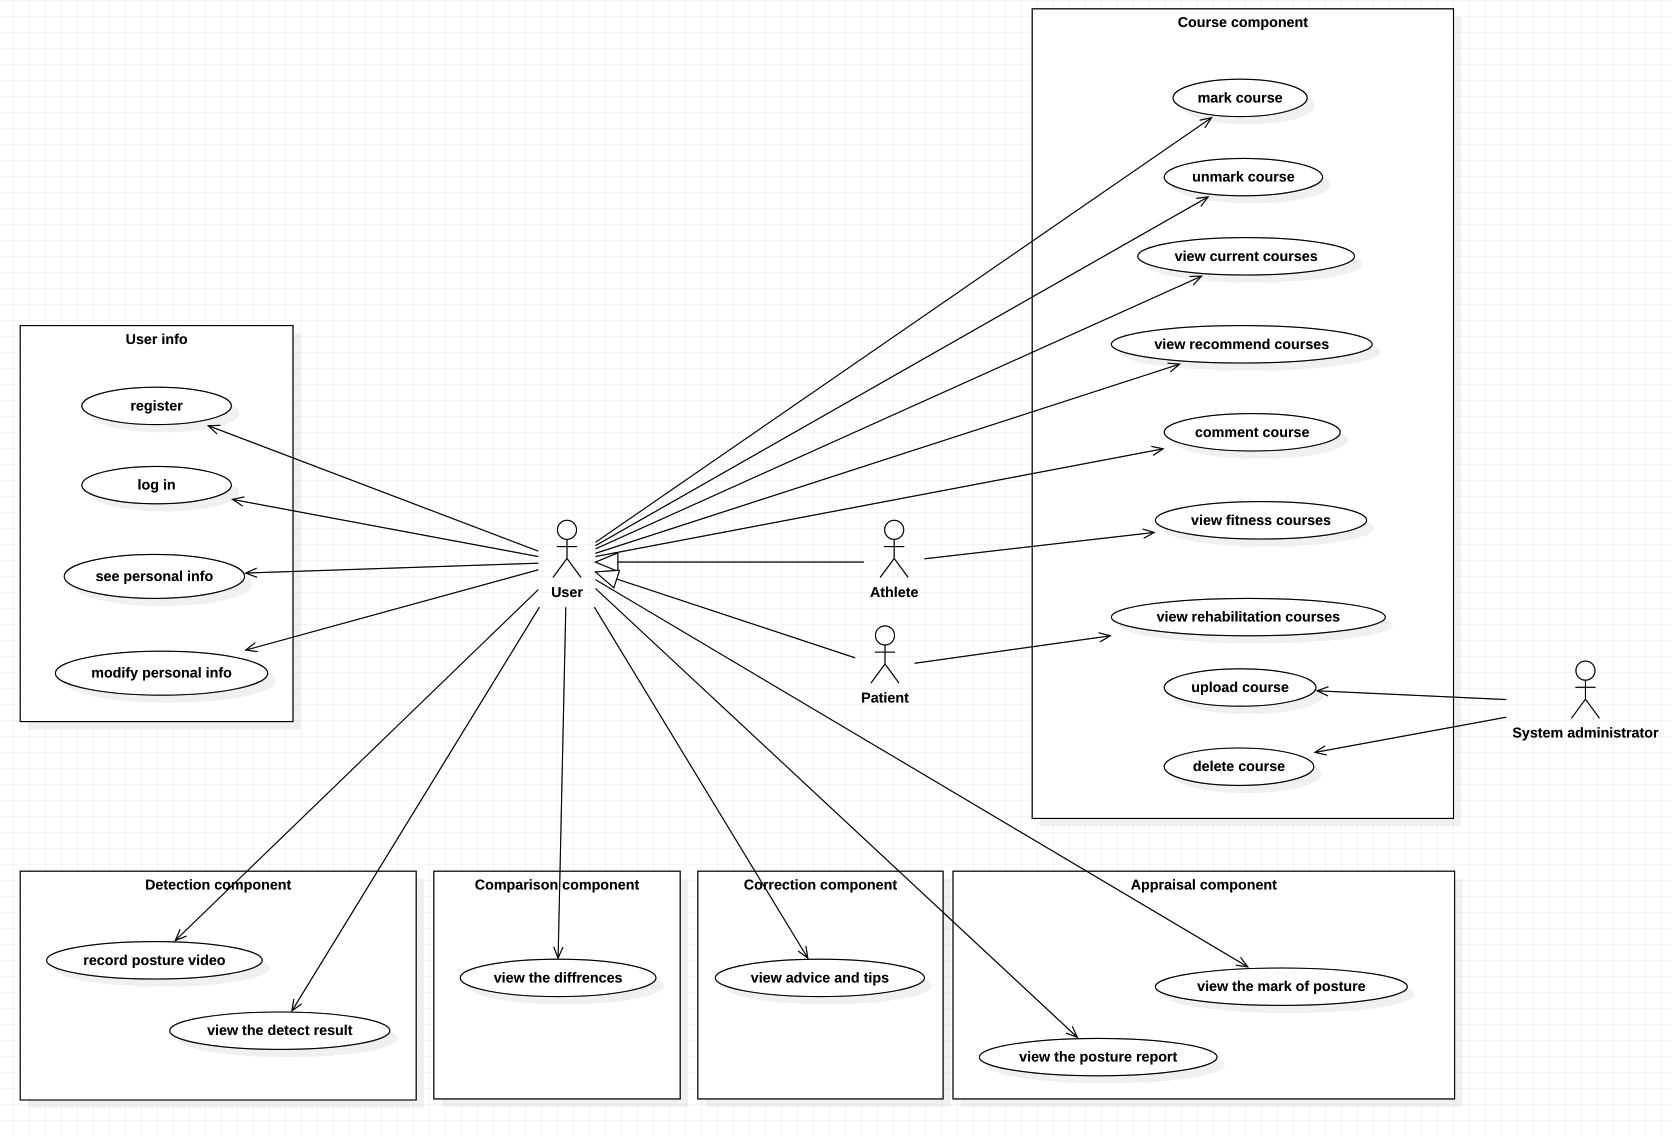
\includegraphics[width=1.0\textwidth]{figures/big-user-case.png}
	\caption{overall user-case diagram}
\end{figure}

\begin{figure}[H]
	\centering
	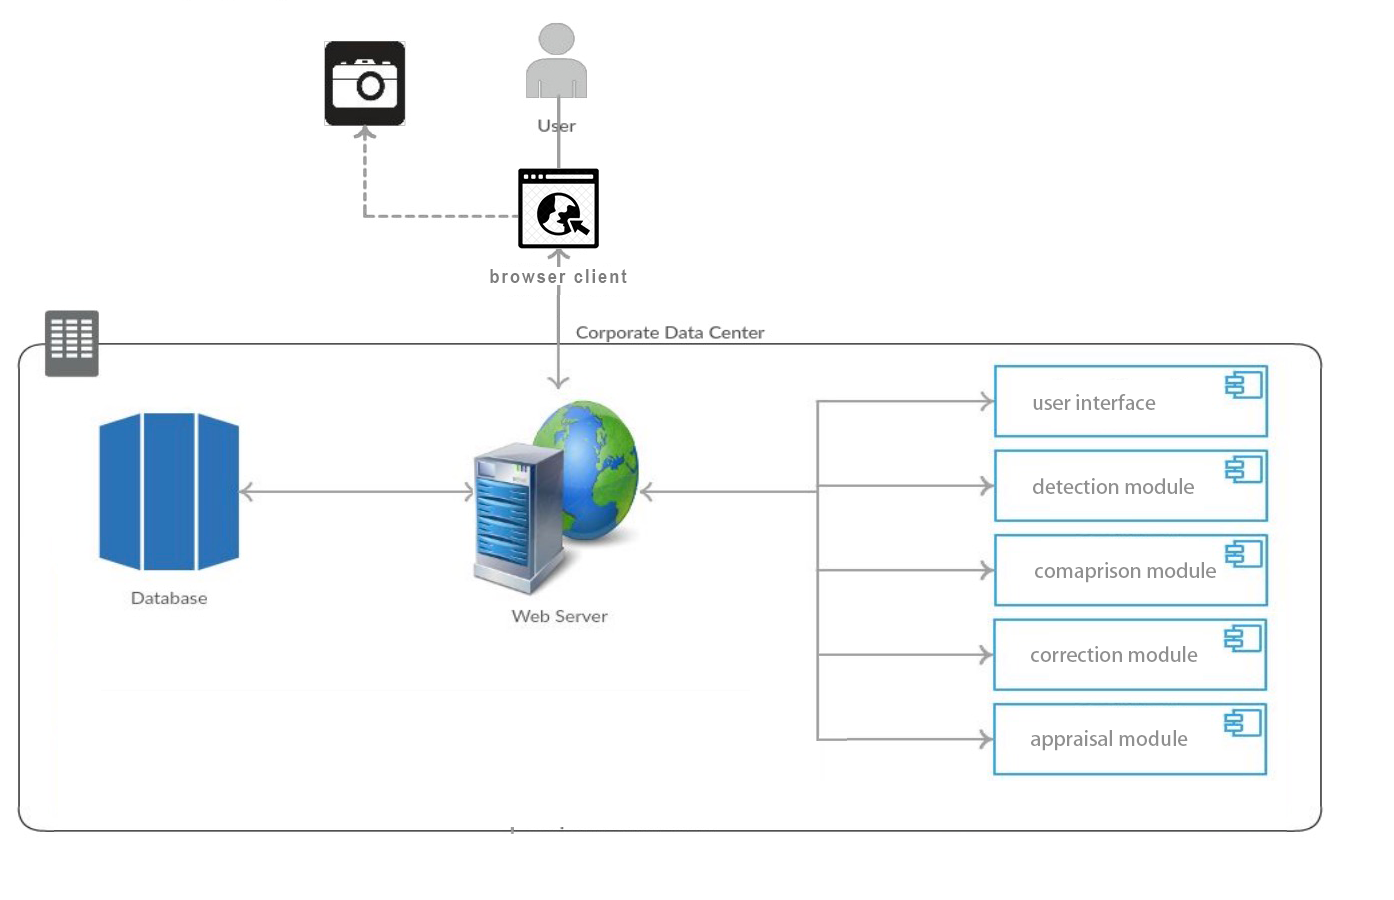
\includegraphics[width=1.0\textwidth]{figures/architecturediagram.png}
	\caption{overall architecture diagram}
\end{figure}

\section{Product Functionality}

ISport contains these following key features:\\
Let the user register their account of the website through their mobile phone or e-mail.\\

 
Let the user log in to the system by correctly complete the log-in form. If the username is not in the database, the user will be prompted to register his/her account.\\

 
User can modify his/her account information after logging in, including the username, e-mail address, phone number, gender, age and so on.\\

 
Show all the sorted fitness courses in a list for user to choose in the fitness courses view page. \\

 
Show a list of courses that the user has selected to learn before\\

 
Show a list of recommended courses for the user by user's previous behavior \\

 
Show the comment and evaluation of each courses in their detailed page\\

 
Provide the add button for user to add a course he/she want to learn in the future and add the course to his/her courses list.\\

 
Provide the delete button for user to remove a course he/she doesn't want to learn and remove the course from his/her courses list.\\


Generate user's exercise report for watching and analyzing in the report page\\
 
Give the user a space to leave his/her evaluation about the courses learnt before\\

Capture and Collect the posture data of the user in front of the computer and store the data in the server.\\


Compare user's posture with the standard one and calculate the similarity between the postures.\\


Show tips on the user's screen to notice the wrong posture of the user and help to correct them.\\


Rate the user's posture on a scale of zero to ten to let the user know whether his posture is standard or not\\


System administrator can upload new courses to the system for users to choose and learn.\\

\section{Users and Characteristics}

 
\begin{center}
    \begin{tabular}{p{5cm}p{11cm}}
        \hline
	    Users & Desc\\
        \hline
	    People who want to correct their posture &  Normal user is expected to register and log in the system, upload their posture and get the feedback advice from the system\\
        \hline
	    People who want to be fitness & People who want to be fitness is expected to register and log in the system, choose fitness classes for themselves and learn it on the website\\
        \hline
        People who need rehabilitation & People who need rehabilitation is expected to register and log in the system, choose fitness classes for themselves and learn it on the website\\
        \hline
        System Administrator & System Administrator has the privilege to update posture information in the database. The Administrator does not directly interact with the website\\
        \hline
    \end{tabular}
\end{center}

 
\section{Operating Environment}

 
\subsubsection{Hardware}

 
\noindent1. Server\\

 
CPU: Intel Dual-Core 2.4GHz\\

 
Memory: 8GB\\

 
External Storage: 500G SSD\\

 
Quantity: 1\\

 
\noindent 2. Client(Minimum Configuration)\\

 
CPU: Single-Core 1GHz\\

 
Memory: 2G\\

 
External Storage: 20GB HDD\\

 
\subsubsection{Software}

 
\noindent 1. Server\\

 
Operating System: Ubuntu 18.04 LTS\\

 
Database: MySQL\\

 
Software and Library : Python, Spring, TensorFlow, Nginx\\

 
\noindent 2. Client\\

 
Operating System: Windows/macOS/Linux/Android/IOS\\

 
Software: Browser\\

 
\begin{center}
    \begin{tabular}{p{7cm}p{7cm}}
        \hline
	    Recommand Browser & Version\\
        \hline
	    Google Chrome &  44+\\
        \hline
	    Mozilla Firefox & 40+\\
        \hline
        Apple Safari & 7+\\
        \hline
        Microsoft Edge & 12+\\
        \hline
        Microsoft Internet Explorer & 11+\\
        \hline
        Opera Opera & 31+\\
        \hline

 
    \end{tabular}
\end{center}

 
\section{Design and Implementation Constraints}

 
\noindent 1. Memory: Server will have 500GB internal hard drive. Softwares and database cannot exceed this amount. System administrator must notice this limitation. And each user should follow the rule that the video data uploaded each time shall not be greater than 100M\\

 
\noindent 2. Language requirements: software must be multilingual, including the following languages: English, Chinese\\

 
\noindent 3. Number of user: each video uploaded must be one person. Each time this system can only deal with one person's data.\\

 
\section{User Documentation}

 
Along with this system: iSport, a user manual need to be written to help users understand how to operate the system. It would be written for nontechnical individuals and the level of content would differ considerably from a system administration guide, which is more detailed and complex. The user manual would follow common user documentation styles to be simple.\\

 
Trying to use step-by-step instructions for users who firstly log in to the website, by showing messaging structures, quick references, tips and glossary of terms.\\

 
User document can be written in HyperText Markup Language (HTML) or Portable Document Format (PDF) , which must describe the use of the software system.

 
\section{Assumptions and Dependencies}

 
It is assumed that the website will work correctly with every third-party operating
system and compatible across all of the major browsers.\\

 
Assumed that the web server always runs well without down or not responding.\\

 
ISport provides two kinds of classes for user to choose: fitness classes and rehabilitation classes.\\

 
Website visitors who have not been registered are only allowed to watch some demo videos, they are not allowed to upload their posture video data before registering.\\

 
In addition to test their posture and attend into courses, members are also allowed to update their information, but they have to log in first.\\


\chapter{Specific Requirements}
\label{Specific Requirements}
\section{External Interfaces Requirements}
\subsection{User Interfaces}
\begin{itemize}
    \item GUI Standard: Material Design is a design language that Google developed in 2014. Expanding on the "card" motifs that debuted in Google Now, Material Design uses more grid-based layouts, responsive animations and transitions, padding, and depth effects such as lighting and shadows.
    \item font Standard: Google Sans Font, agree with Material Design
    \item button Standard: Material Design
    \item color scheme: Dark, Light, changes in different system color scheme. Nowadays, every OS has at least 2 types color scheme, someone may prefer dark mode to be less distract.
    \item screen layout/resolution: adapt to user's device
    \item function, navigation links: in login page, user can go to homepage or register page by router. After entering homepage, user can see a navigation bar, in which user can jump to every sub-page without difficulty.
    \item message display: every dangerous change, such as changing password, username, phone number, the web page will show a message notification, on the righttop. If user does some wrong gestures, it will show a message notification and bell a sound to warn.
\end{itemize}
\subsection{Hardware Interfaces}
\begin{itemize}
    \item supported device:\\
        \begin{itemize}
            \item mobile phones, including Android and iOS devices, with camera authorization.
            \item computers with camera or laptop, with camera authorization.
        \end{itemize}

    \item deployed device:\\
        A cloud web server in Ali Cloud, with 4 gigabytes RAM and dual-core CPU and 1TB disk.\\
        We deployed our web service, including database, backend on one server, the user amount now is not a large number, in some day if the user group grows larger and larger, we may use multiple servers and consider disturbed system.  
\end{itemize}
    Our product recall the interface between camera, to update data which contains the gestures user does to our server to analysis whether what the user does corresponds to criterion.
\subsection{Software Interfaces}
\begin{itemize}
    \item Third part APIs we use
        \begin{itemize}
            \item OS: our service requires the OS grant the permission to recall camera of user divices.
            \item database: the database of our service is generally MySQL. Java Database Connectivity (JDBC) is an application programming interface (API) for the programming language Java, which defines how a client may access a database. It is a Java-based data access technology used for Java database connectivity. It is part of the Java Standard Edition platform, from Oracle Corporation. It provides methods to query and update data in a database, and is oriented towards relational databases. A JDBC-to-ODBC bridge enables connections to any ODBC-accessible data source in the Java virtual machine (JVM) host environment. To make jwt works correctly, we use a key-value dababase called redis, storing outdated token and blocking them to avoid a situation that a user just changed his password, but his token is still not outdated, because jwt cannot forces a token to be outdated.
            \item Springboot: the backend programm language is Java, our backend is based on Springboot and developed in form of microservice architecture. Microservice architecture is a development trend and arranges an application as a collection of loosely coupled services. In a microservices architecture, services are fine-grained and the protocols are lightweight. With APIs provided by Springboot, the development goes efficiently and standard.
            \item PoseNet: our identification technologies is provided by a open-source project named PoseNet, PoseNet contains a standalone model called PoseNet, as well as some demos, for running real-time pose estimation in the browser using TensorFlow.js.
        \end{itemize}
    \item APIs we provide
        \begin{itemize}
            \item user register API\\
                This API provides the function that a new user becomes a new menber of iSport.\\
                API checks:
                \begin{itemize}
                    \item whether the username has registered, 
                    \item whether the phone or email is empty
                \end{itemize}
                if pass all restrict, the new user owns his data in our database.
            \item user login API\\
                This API provides the function that a user launch a new session.\\
                API checks:
                \begin{itemize}
                    \item whether this user has register.
                    \item the correction of password
                \end{itemize}
                if pass all restrict, the user now has logged in. He can begin to exercise.
            \item all courses API\\
                This API recieves a integer send by client, requests backend to return all courses with the type user type in. There two types of courses in iSport, one is rehabilitation course and the other is training course.
                API checks the type typed in by user, an integer, to return. Only 0 and 1 is valid, 1 is for rehabilitation, and 0 is for training.
            \item course content API\\ 
                This API recieves an ID of a course, and return all photography of this course, the provide a basic message to users.\\
                API checks the input, make sure that the input is not an empty input, then query in database, if the ID is invalid(e.g. not a course with this ID), the API throw an exception. If not, API respond with all photography about this course in database.
            \item get user name\\
                This API revives the ID of user, returns the username.\\
                API checks the validity of the input, if the ID is valid, API respond with the username.
            \item get user information\\
                This API recieves the ID of user, returns the user information.\\
                API checks the validity of the input, if the ID is valid, API respond with all user information.
            \item update the user information\\
                This API recieves the ID and information to update, to update user information in the database.\\
                API checks the validity of input, if ID is invalid, or one of all the parameter is empty, the API throws an exception.
            \item course information\\
                This API need the login data of user. Requests backend to respond all courses the user has taken.
            \item course delete\\
                This API need the login data of user. send the id of the course to be deleted, requests backend to delete this course information in user's take table.
                If the user doesn't take this course, this API throws an exception.
        \end{itemize}
\end{itemize}
\subsection{Communications Interfaces}
The data transferring in the Internet is video, and we choose the broadcast protocol is http-flv. This protocol is widely ued in the living industry, with the advantage of low-delay and ease to go through the firewall, it is also friendly to dispatch the rate of flow. \\ 
The session communication data is transferred in form of json. Json is a lightweight data-interchange format. It is easy for humans to read and write. It is easy for machines to parse and generate. Using jwt to authenticate can confirm safety of user session data. JSON Web Token (JWT) is an Internet standard for creating JSON-based access tokens that assert some number of claims. For example, a server could generate a token that has the claim "logged in as admin" and provide that to a client. The client could then use that token to prove that it is logged in as admin. The tokens are signed by one party's private key (usually the server's), so that both parties (the other already being, by some suitable and trustworthy means, in possession of the corresponding public key) are able to verify that the token is legitimate. The tokens are designed to be compact, URL-safe, and usable especially in a web-browser single-sign-on (SSO) context. JWT claims can be typically used to pass identity of authenticated users between an identity provider and a service provider, or any other type of claims as required by business processes. \\
%\section{User Interfaces}
%$<$Describe the logical characteristics of each interface between the software 
%product and the users. This may include sample screen images, any GUI standards 
%or product family style guides that are to be followed, screen layout 
%constraints, standard buttons and functions (e.g., help) that will appear on 
%every screen, keyboard shortcuts, error message display standards, and so on.  
%Define the software components for which a user interface is needed. Details of 
%the user interface design should be documented in a separate user interface 
%specification.$>$

\clearpage
\section{Functional Requirements}

\subsection{Functional Modeling}
\begin{figure}[H]
    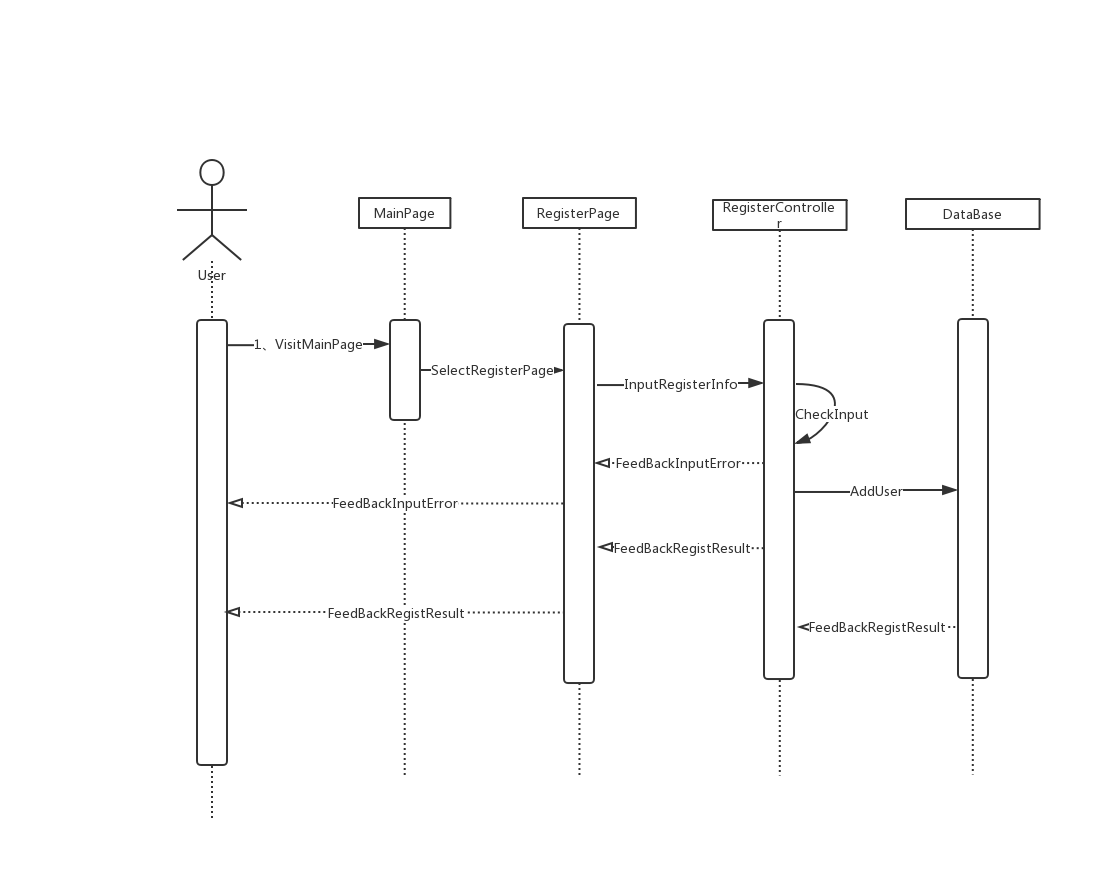
\includegraphics[width=\linewidth]{./FuncPhoto/1.png}   
    \caption{Register}
\end{figure}
User should register before he uses our service. Function will ensure that the input is legal and not exists in database.

\begin{figure}[H]
    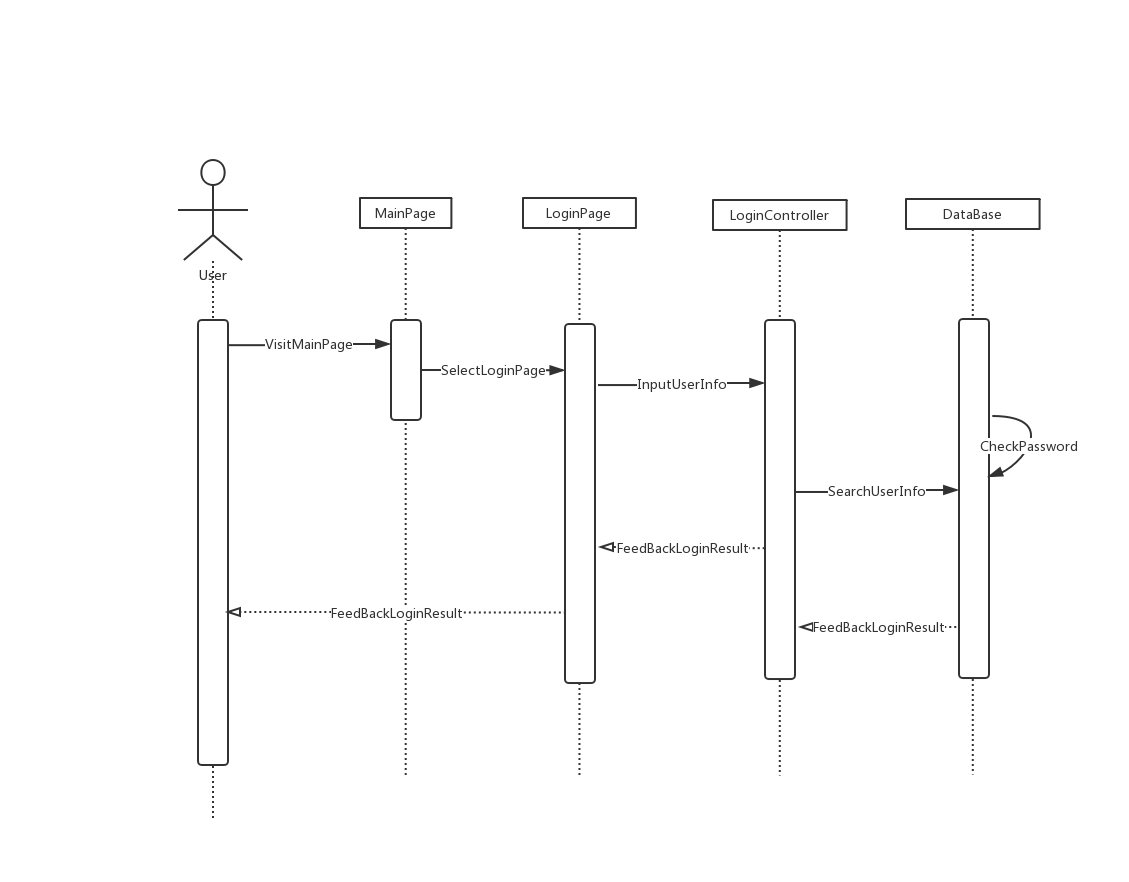
\includegraphics[width=\linewidth]{./FuncPhoto/2.png}   
    \caption{Login}
\end{figure}
User should log in before he uses our service. 

\begin{figure}[H]
    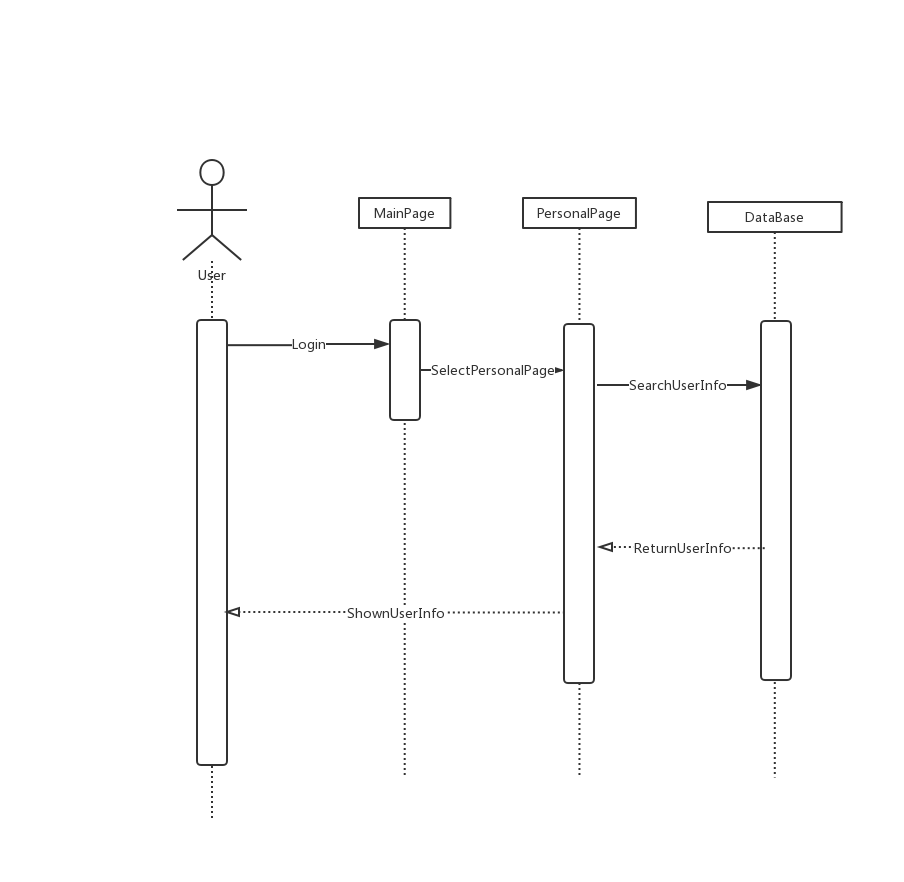
\includegraphics[width=\linewidth]{./FuncPhoto/3.png}   
    \caption{Display User Info}
\end{figure}
The user information is displayed in user interface, such as username, user's course. Frontend will recall this API after logging in.

\begin{figure}[H]
    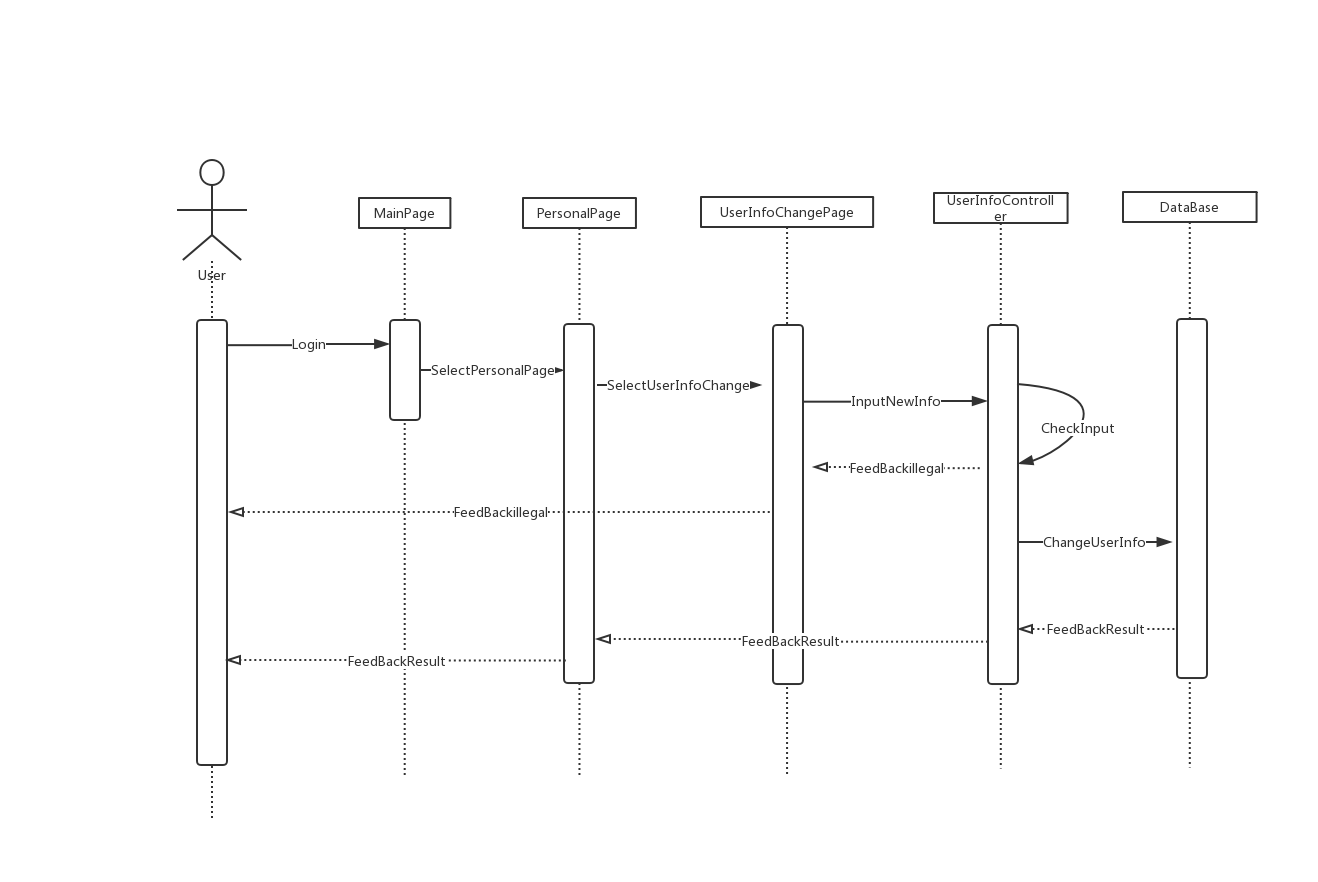
\includegraphics[width=\linewidth]{./FuncPhoto/4.png}   
    \caption{modify User Info}
\end{figure}
A user can modify his information, such as phone number, email address, username or password, anything but user ID. User identification should be checked once he requests a modification.

\begin{figure}[H]
    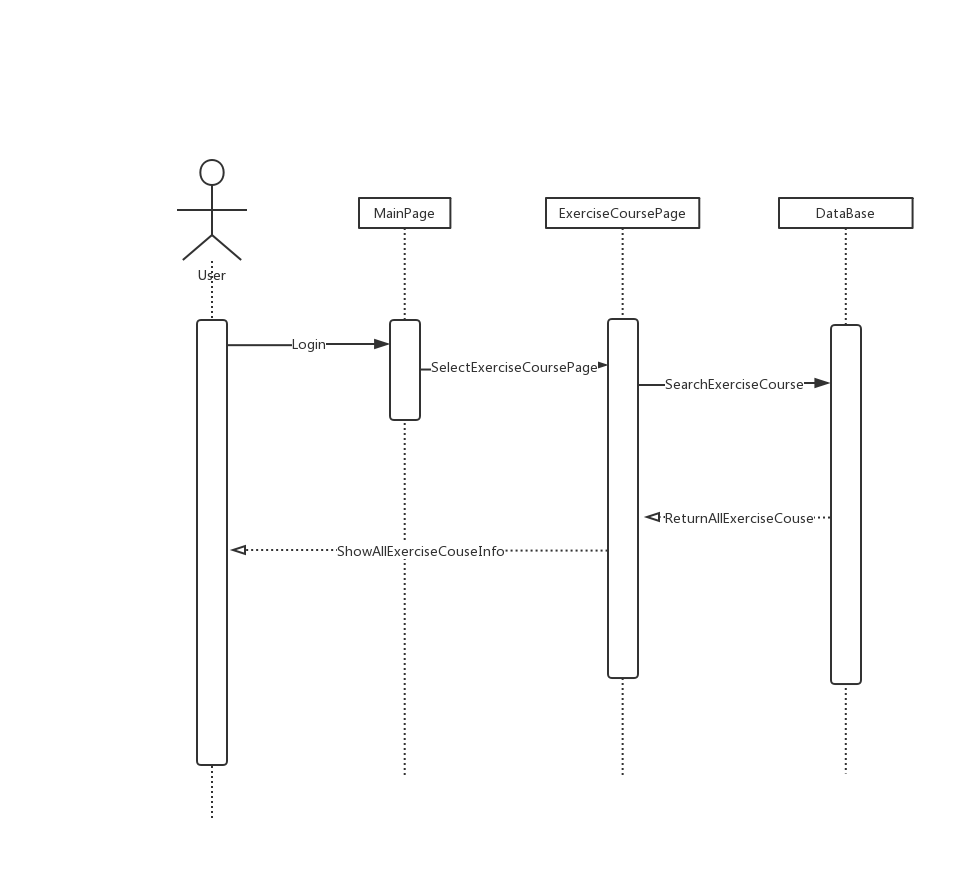
\includegraphics[width=\linewidth]{./FuncPhoto/5.png}   
    \caption{Display Exercise Course}
\end{figure}
User can browse all course he has taken, then choose one to go on with. This API is for exercise courses.

\begin{figure}[H]
    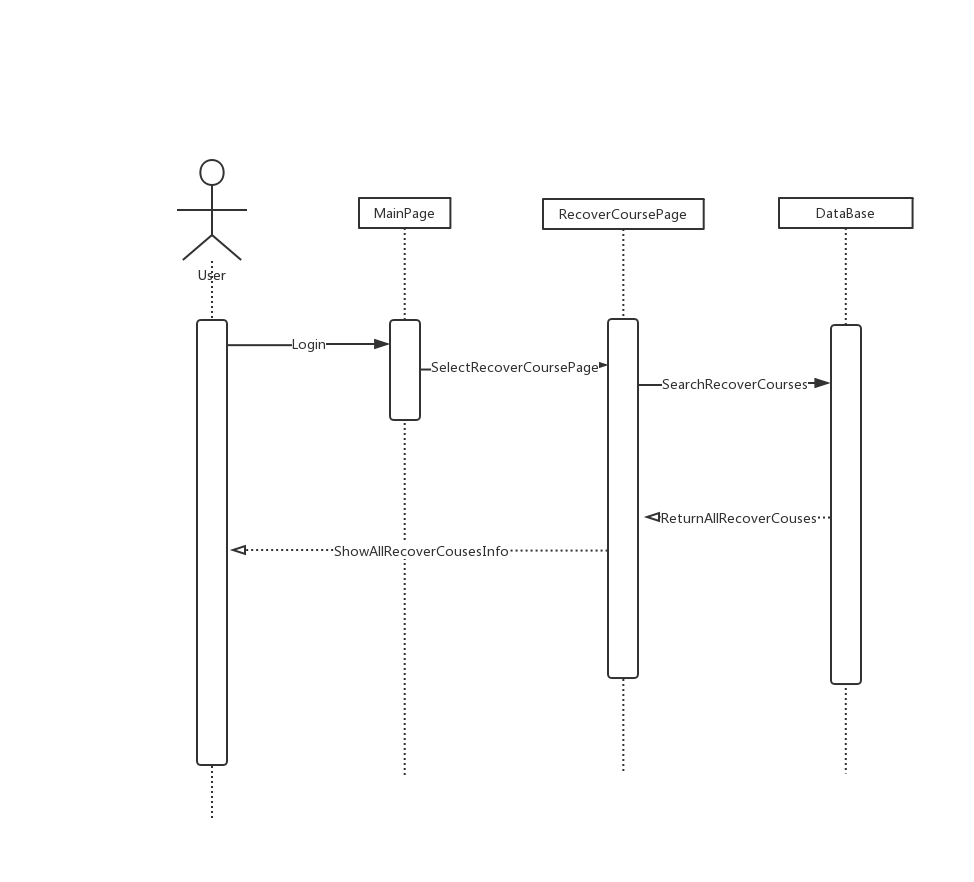
\includegraphics[width=\linewidth]{./FuncPhoto/6.png}   
    \caption{Display Recover Course}
\end{figure}
User can browse all course he has taken, then choose one to go on with. This API is for recover courses. 

\begin{figure}[H]
    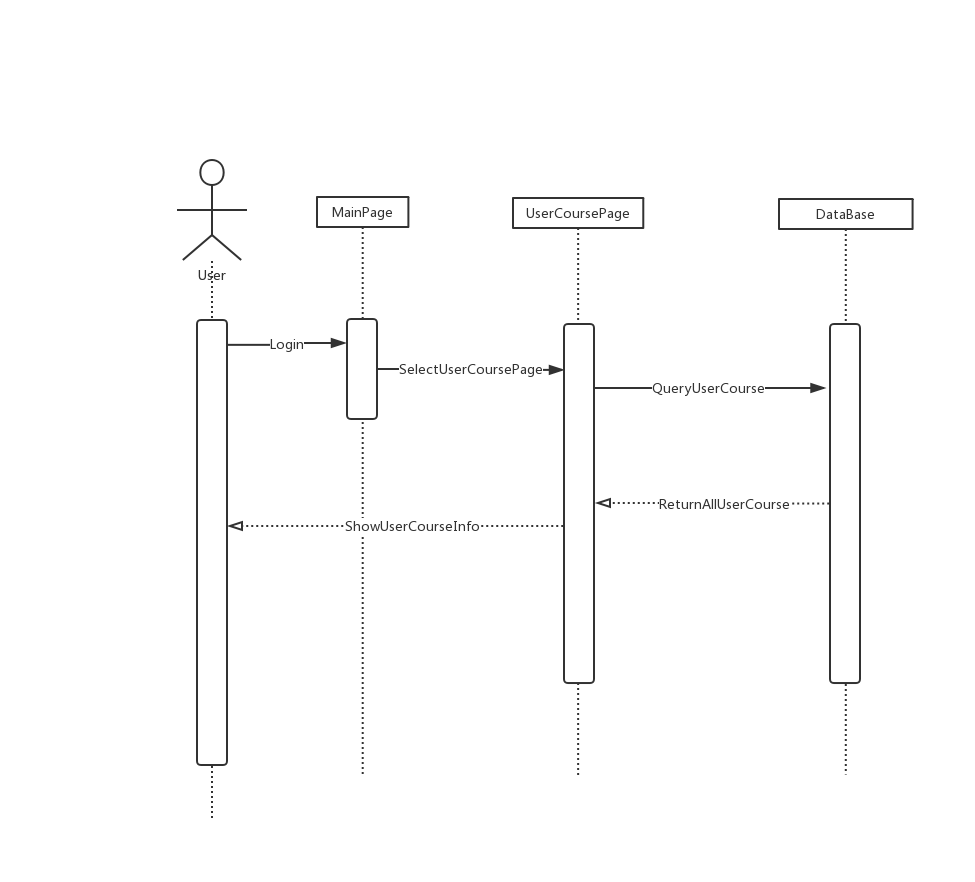
\includegraphics[width=\linewidth]{./FuncPhoto/7.png}   
    \caption{Display User Courses}
\end{figure}
User can browse all course he has taken, then choose one to go on with. This API is for all courses. 

\begin{figure}[H]
    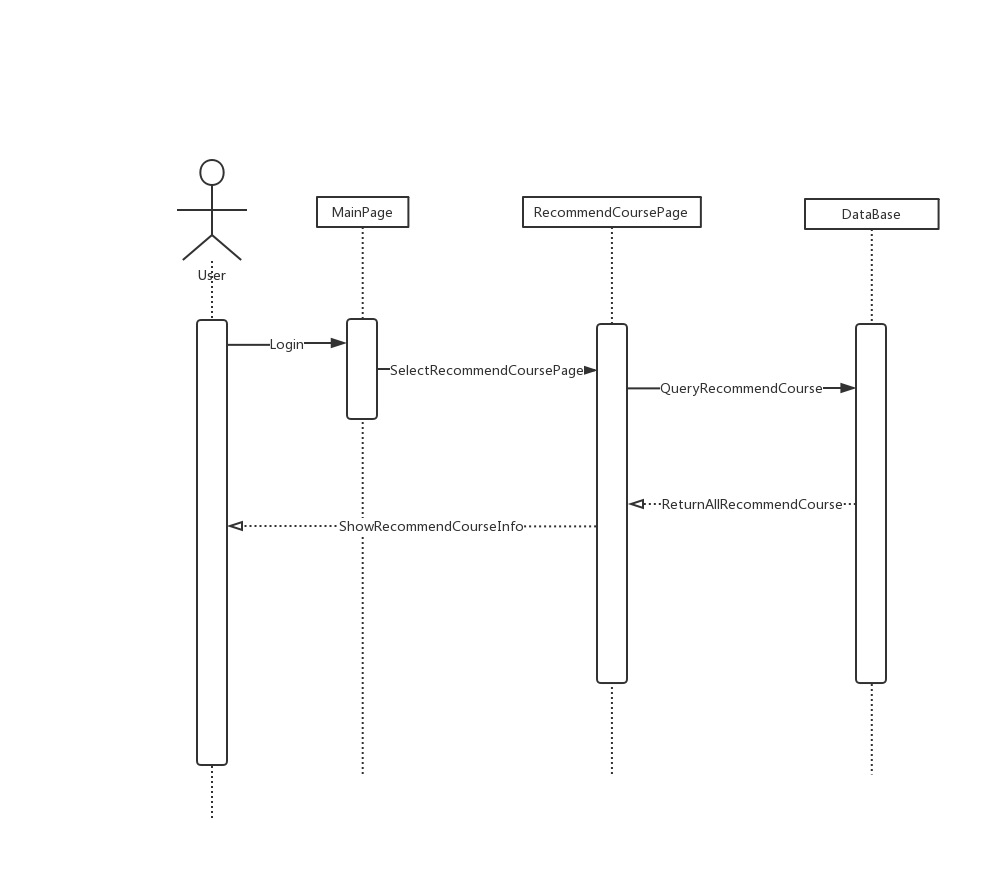
\includegraphics[width=\linewidth]{./FuncPhoto/8.png}   
    \caption{Display Recommend Courses}
\end{figure}
Sometimes user need our system to give some recommends on courses. The recommend system is based on user's course which he has taken.

\begin{figure}[H]
    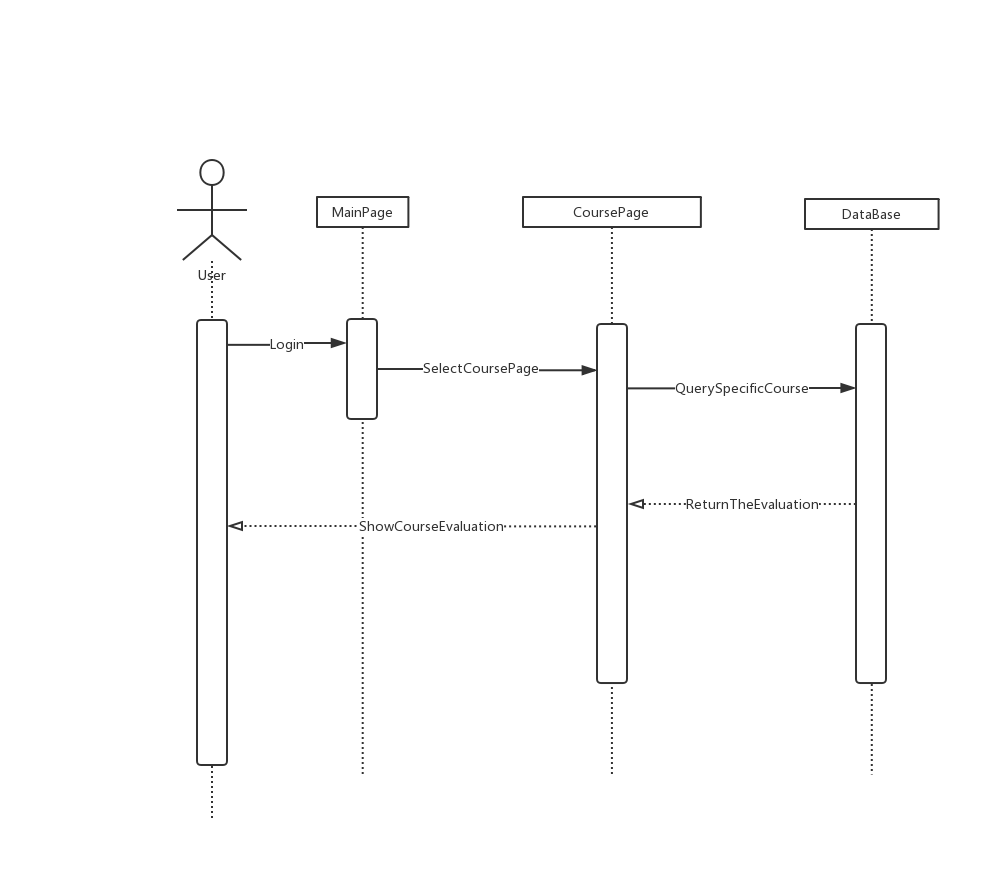
\includegraphics[width=\linewidth]{./FuncPhoto/9.png}   
    \caption{Display Course Evaluation}
\end{figure}
Before user takes a course, he may browse the evaluation to judge whether a course is worth taking.

\begin{figure}[H]
    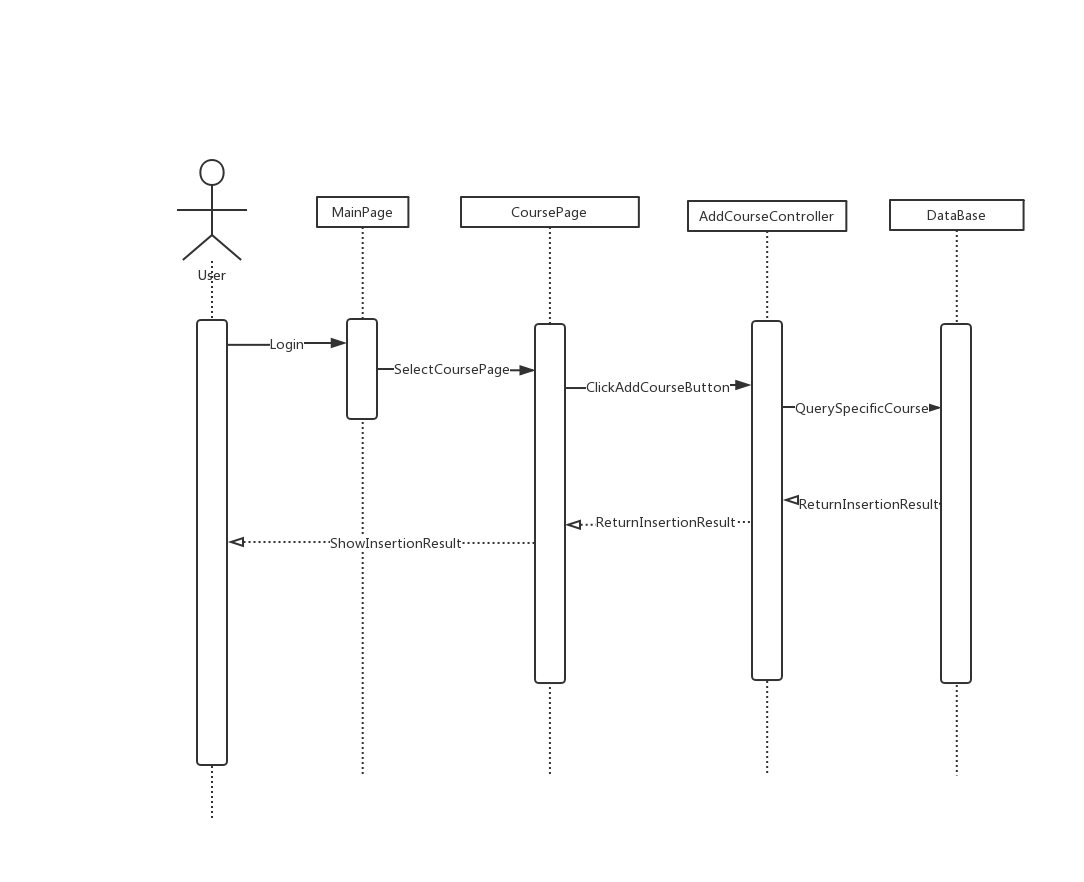
\includegraphics[width=\linewidth]{./FuncPhoto/10.png}   
    \caption{Add to My Course}
\end{figure}
User can add a favored course to his course list. He can browse his favored course in user center.

\begin{figure}[H]
    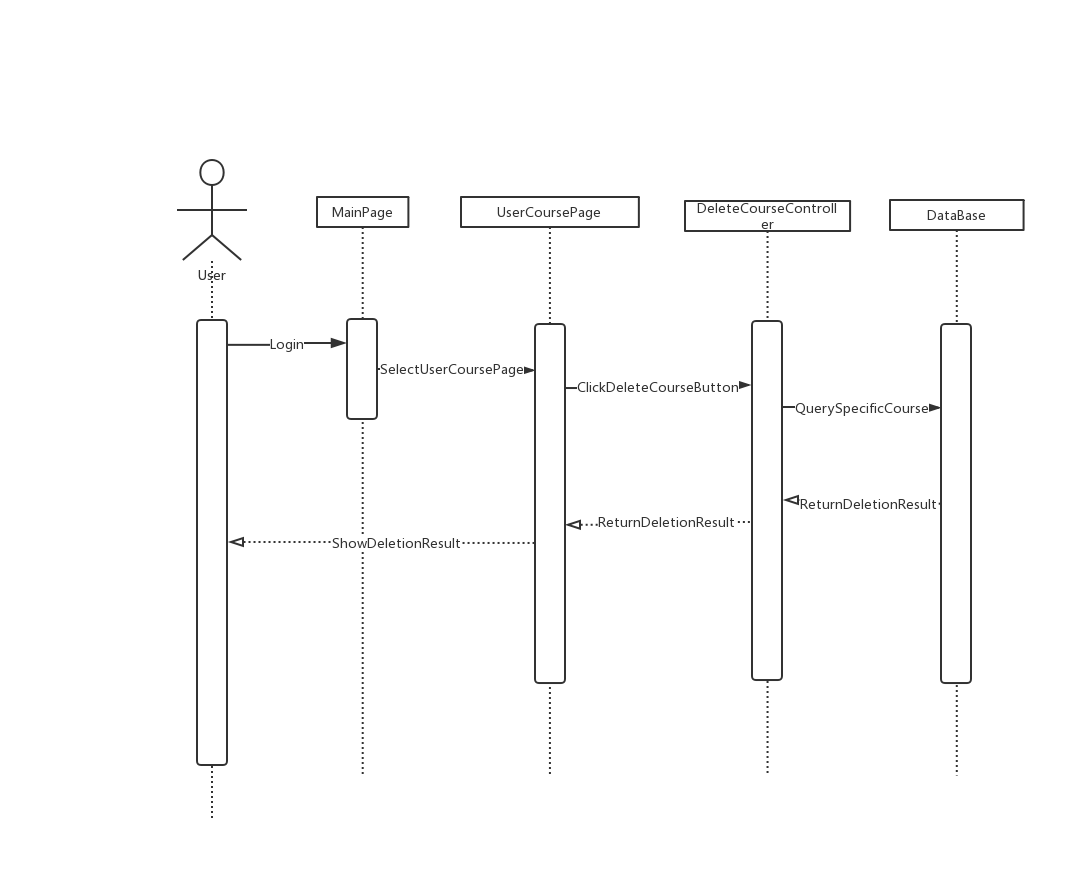
\includegraphics[width=\linewidth]{./FuncPhoto/11.png}   
    \caption{Delete from My Course}
\end{figure}
If User decide not to take a course any more, he can delete a unwished course from his course list.

\begin{figure}[H]
    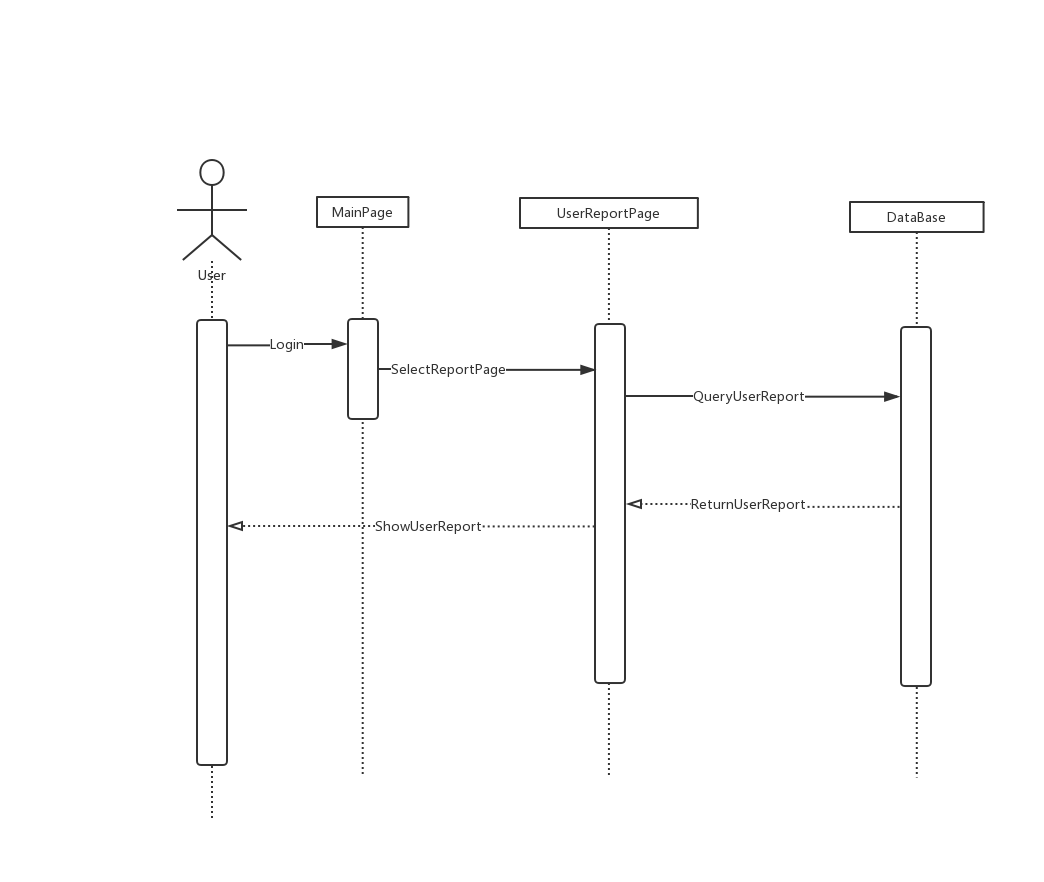
\includegraphics[width=\linewidth]{./FuncPhoto/12.png}   
    \caption{Display User Report}
\end{figure}
A coach may review course takers' report to modify his course, make it more reliable.

\begin{figure}[H]
    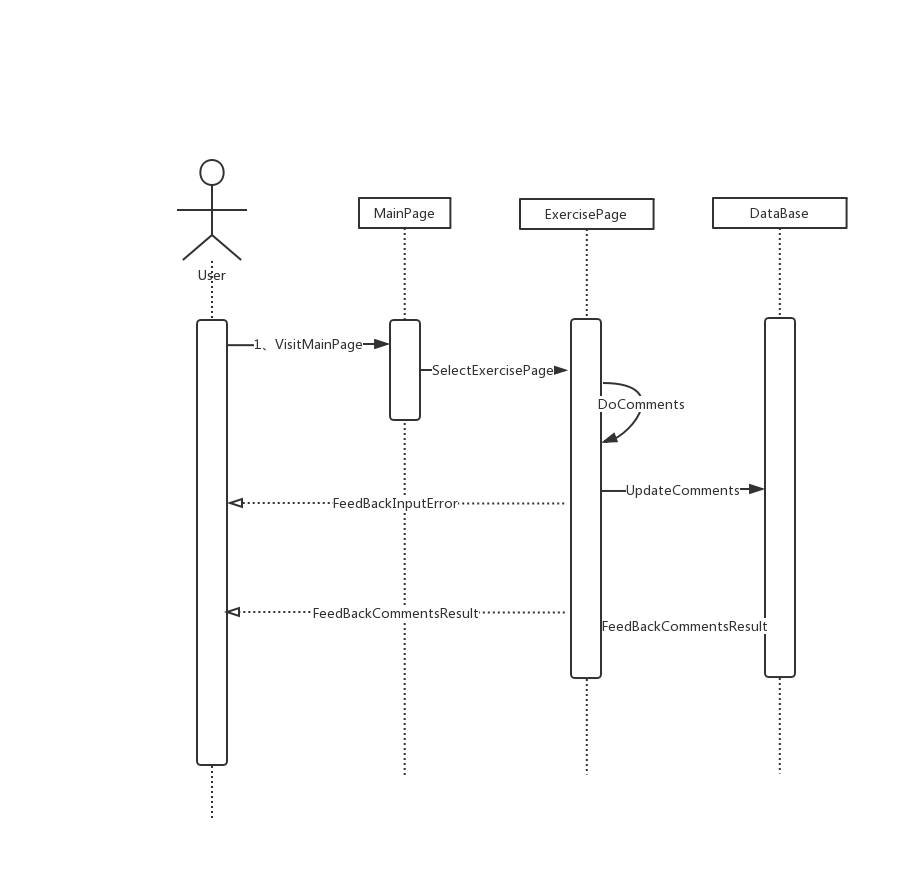
\includegraphics[width=\linewidth]{./FuncPhoto/13.png}   
    \caption{Comment Courses}
\end{figure}
User can comment courses he takes. The comment will be shown on a forum, users can communicate with each other.

\begin{figure}[H]
    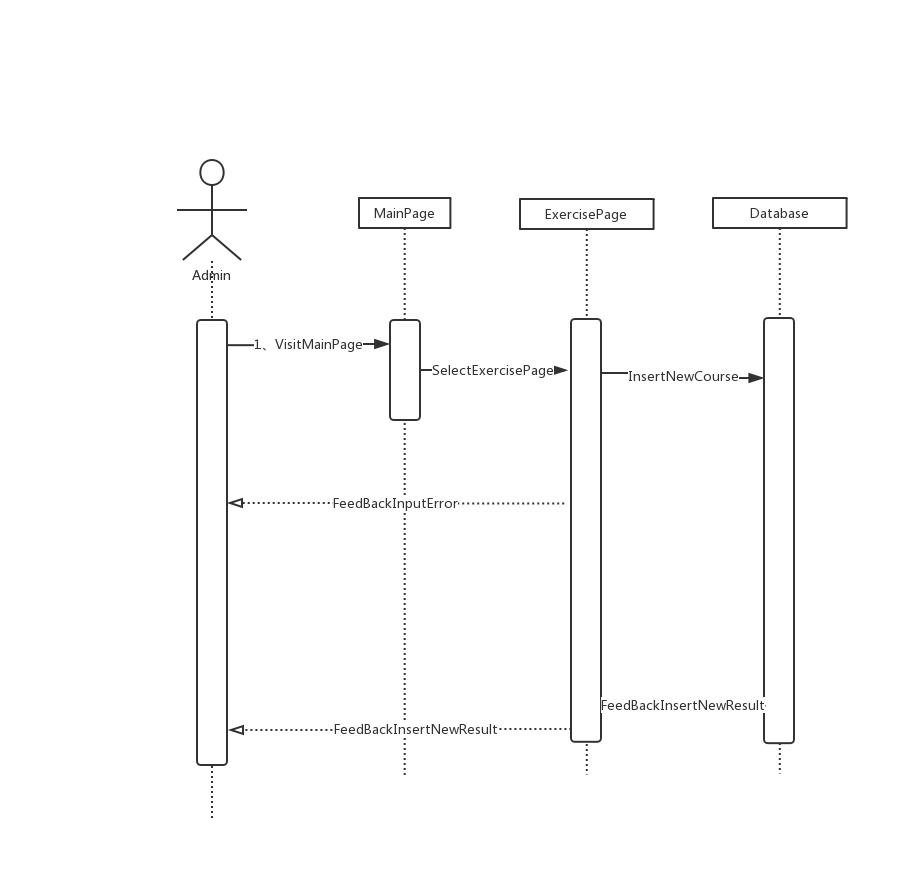
\includegraphics[width=\linewidth]{./FuncPhoto/14.png}   
    \caption{Collect Gesture Data}
\end{figure}
System collects user's gesture data to analyze. The data will only be used for analyzing whether user does is wrong. 

\begin{figure}[H]
    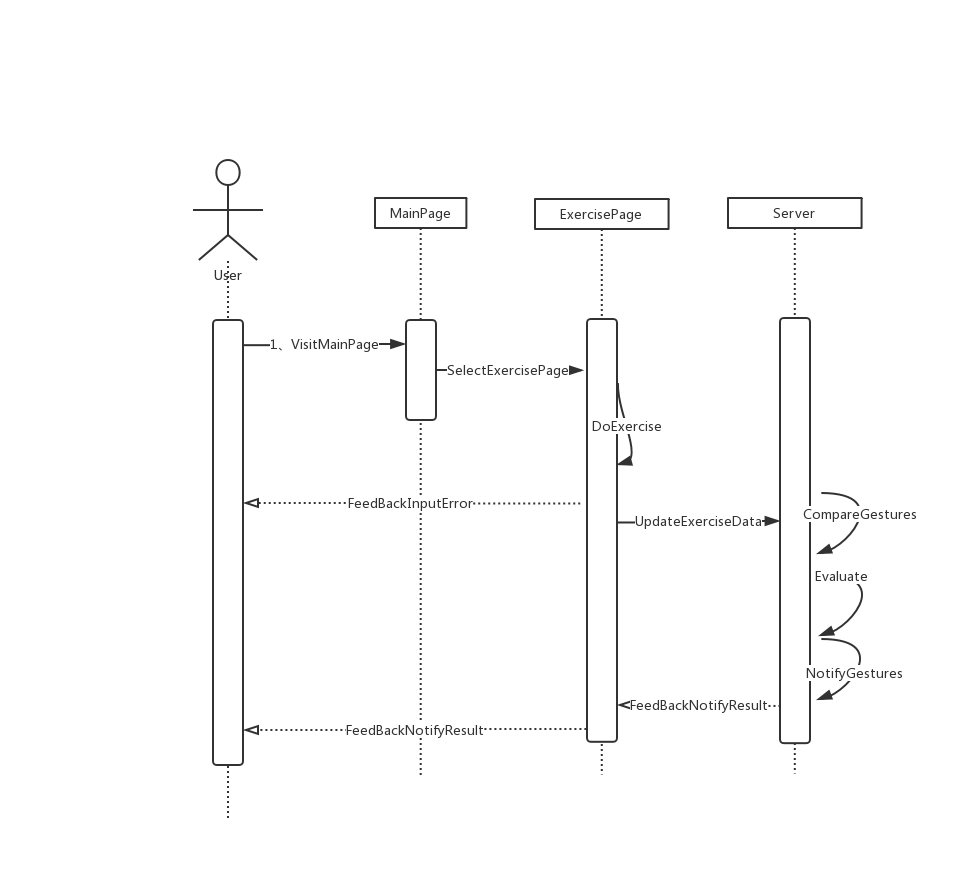
\includegraphics[width=\linewidth]{./FuncPhoto/15.png}   
    \caption{Compare Gesture Data}
\end{figure}
System compare user's gesture data with coach's. If dismatched, a notification will be generated, and system will send it to user's end.

\begin{figure}[H]
    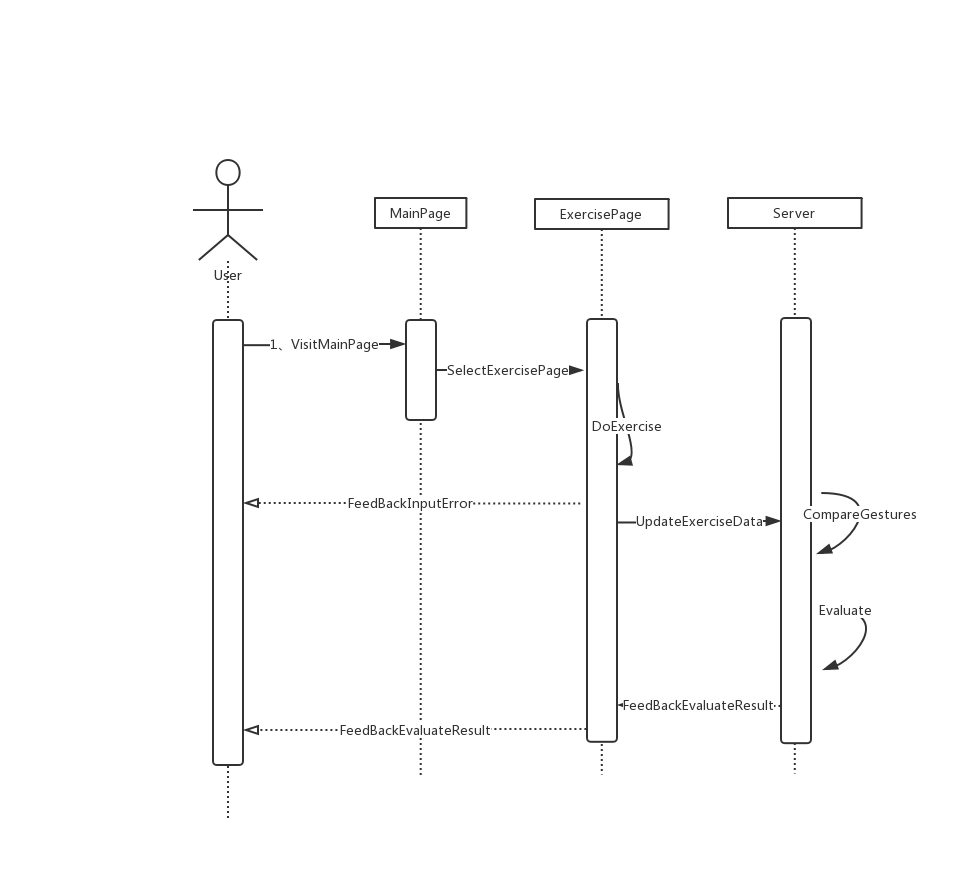
\includegraphics[width=\linewidth]{./FuncPhoto/16.png}   
    \caption{Notify Discrepancy Gesture }
\end{figure}
If the user did wrong, System generate a notification and send to user's browser, user can get a wain fron backend and knoew what he does is wrong.

\begin{figure}[H]
    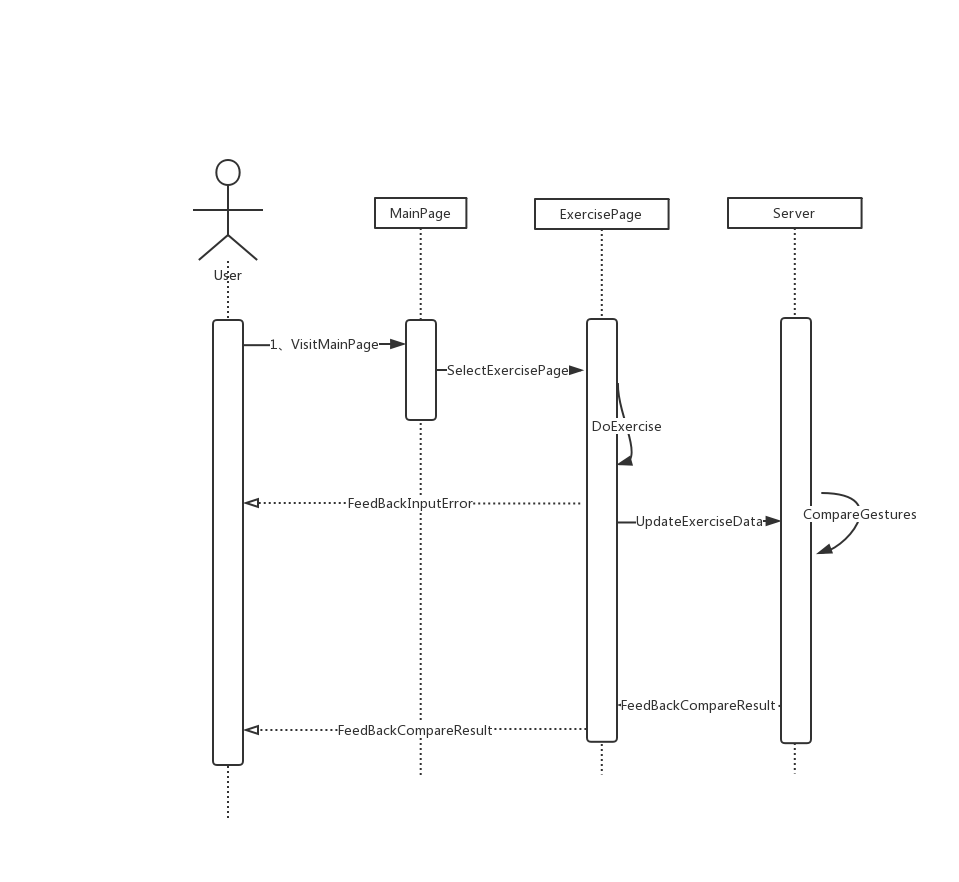
\includegraphics[width=\linewidth]{./FuncPhoto/17.png}   
    \caption{Evaluate Courses}
\end{figure}
After user learns a course, user can evaluate a course by his learning achievement. If user dislikes this course, he can also submit a negative evaluation.

\begin{figure}[H]
    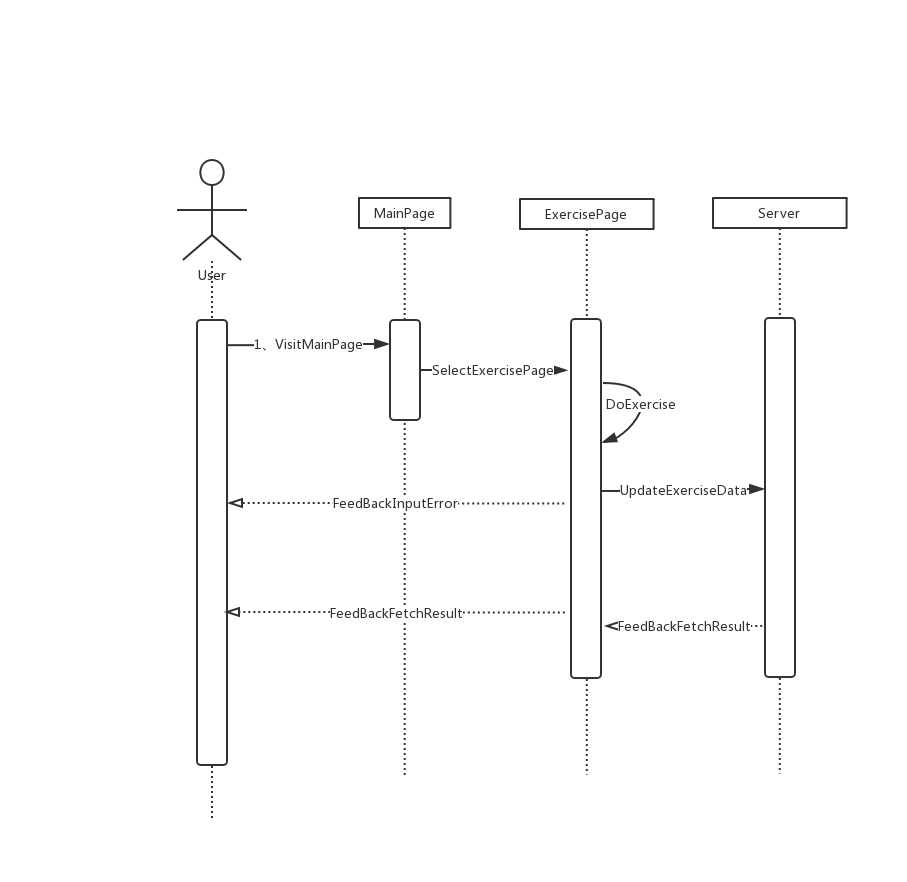
\includegraphics[width=\linewidth]{./FuncPhoto/18.png}   
    \caption{Add New Courses}
\end{figure}
The courses data need be keeped updating. A coach, most of the time an administrator can add new courses to dababase. After auditing, the course will be displayed on our website. 
 
\subsection{Data Modeling}
\subsubsection{Scenario Description}
First, \underline{users} need to register and input their information including \underline{account name}, \underline{password}, \underline{tel-number} and \underline{email address}. For users’ convenience, they can change their \underline{information} in later days.\\
\noindent Only after the user log in, he/she can use the \underline{function} of \underline{iSport}. For \underline{athletes} and \underline{sports fans}, they can view the \underline{exercise course} page and select the one they favor, adding the course to \underline{my course} page. The same is to the \underline{injured patients}, they can go to the \underline{recover course} page and add their favorite courses. Before the users select their \underline{courses}, they can go to the comment page to consider the \underline{comments} given by other users. \\
\noindent When the user decide to start the course, \underline{camera} will open and get the user’s \underline{postures}, meanwhile for \underline{dynamic courses}, the \underline{standard video} will start to play and for \underline{static course}, the \underline{images} will start to switch, then the user have to follow the video’s postures when exercising, at the same time, iSport will notify the user if his/her pass the posture and how to correct their postures. \\
\noindent When the course is finished, user will get a \underline{grade} given by iSport to feedback their performance for the whole course. Of course, they user will get a detailed \underline{report} in report page.

\noindent And for \underline{administrators}, they can upload new course to the iSport database.

\subsubsection{Noun extraction}
\begin{itemize}
	\item User
	\item Account name
	\item Password
	\item Tel-number
	\item Email-address
	\item Function
	\item iSport System
	\item Athletes
	\item Sports fans
	\item Exercise course
	\item Injured patients
	\item Recover course
	\item Comments
	\item Camera
	\item Postures
	\item Standard video
	\item Dynamic course
	\item Images
	\item Static course
	\item Grade
	\item Report
	\item My course
	\item User information
	\item Administrator
\end{itemize}

\subsubsection{Potential Classes}
 Coad and Yourdon[5] lists six selection features for analyzing potential classes which is  referred by Pressman[4]:
 \begin{enumerate}
 	\item Message Keeping
 	\item Services Requiring
 	\item Multiple Attributes
 	\item Public Attributes
 	\item Public Operations
 	\item Necessary Requirements
 \end{enumerate}
 Analysis Table is as follows:
 
\begin{longtable}{|p{1.9in}|p{4in}|c|}
xxxxx & xxxxxx  \kill
\caption{Potential Classes Analysis Table\label{ptable}}\\ \hline
\multicolumn{3}{|c|}{\bf Potential Classes Analysis}\\ \hline
\endfirsthead
\caption[]{(continued)}\\ \hline
\multicolumn{3}{|c|}{\bf Potential Classes Analysis (continued)}\\
\hline
\endhead
\hline
\multicolumn{3}{|c|}{\bf Continued $\ldots$}\\
\hline
\endfoot
\hline
\multicolumn{3}{|c|}{\bf The End}\\
\hline
\endlastfoot
\textbf{Potential Classes} & \textbf{Features Matched}  \\
\hline
User & Accepted: All match\\  \hline  
Account name & Denied: Only matches 1\\ \hline
Password & Denied: Only matches 1\\  \hline
Tel-number & Denied: Only matches 1\\  \hline
Email-address & Denied: Only matches 1\\ \hline
User Info & Denied:Don't match 2,3,4,5,6\\ \hline
Courses & Accepted: Satisfy all.\\ \hline
Exercise Courses & Denied: Only matches 1\\ \hline
Recover Courses & Denied: Only matches 1\\ \hline
Static Courses & Accepted: Satisfy all\\ \hline
Dynamic Courses & Accepted: Satisfy all\\ \hline
iSport System& Don't match any\\ \hline
Function& Denied: Don't match any\\ \hline 
Athletes & Accepted: All match\\ \hline
Sports fans& Accepted: All match\\ \hline 
Sport Report & Accepted: All match\\ \hline 
Injured patients & Accepted: All match\\ \hline 
Comments & Denied: Only matches 1\\ \hline 
Camera & Denied: Only matches 1\\ \hline 
Postures & Denied:Only matches 1\\ \hline 
Standard video & Denied:Only matches 1\\ \hline 
Images & Denied:Only matches 1\\ \hline 
Grade & Denied:Don't match 2,3,4,5,6\\ \hline
My course & Denied:Don't match 2,3,4,5,6\\ \hline 
Administrator & Accepted: All match\\ \hline
\end{longtable}

\subsubsection{Overview Class Diagram}
\begin{figure}[H]
\centering
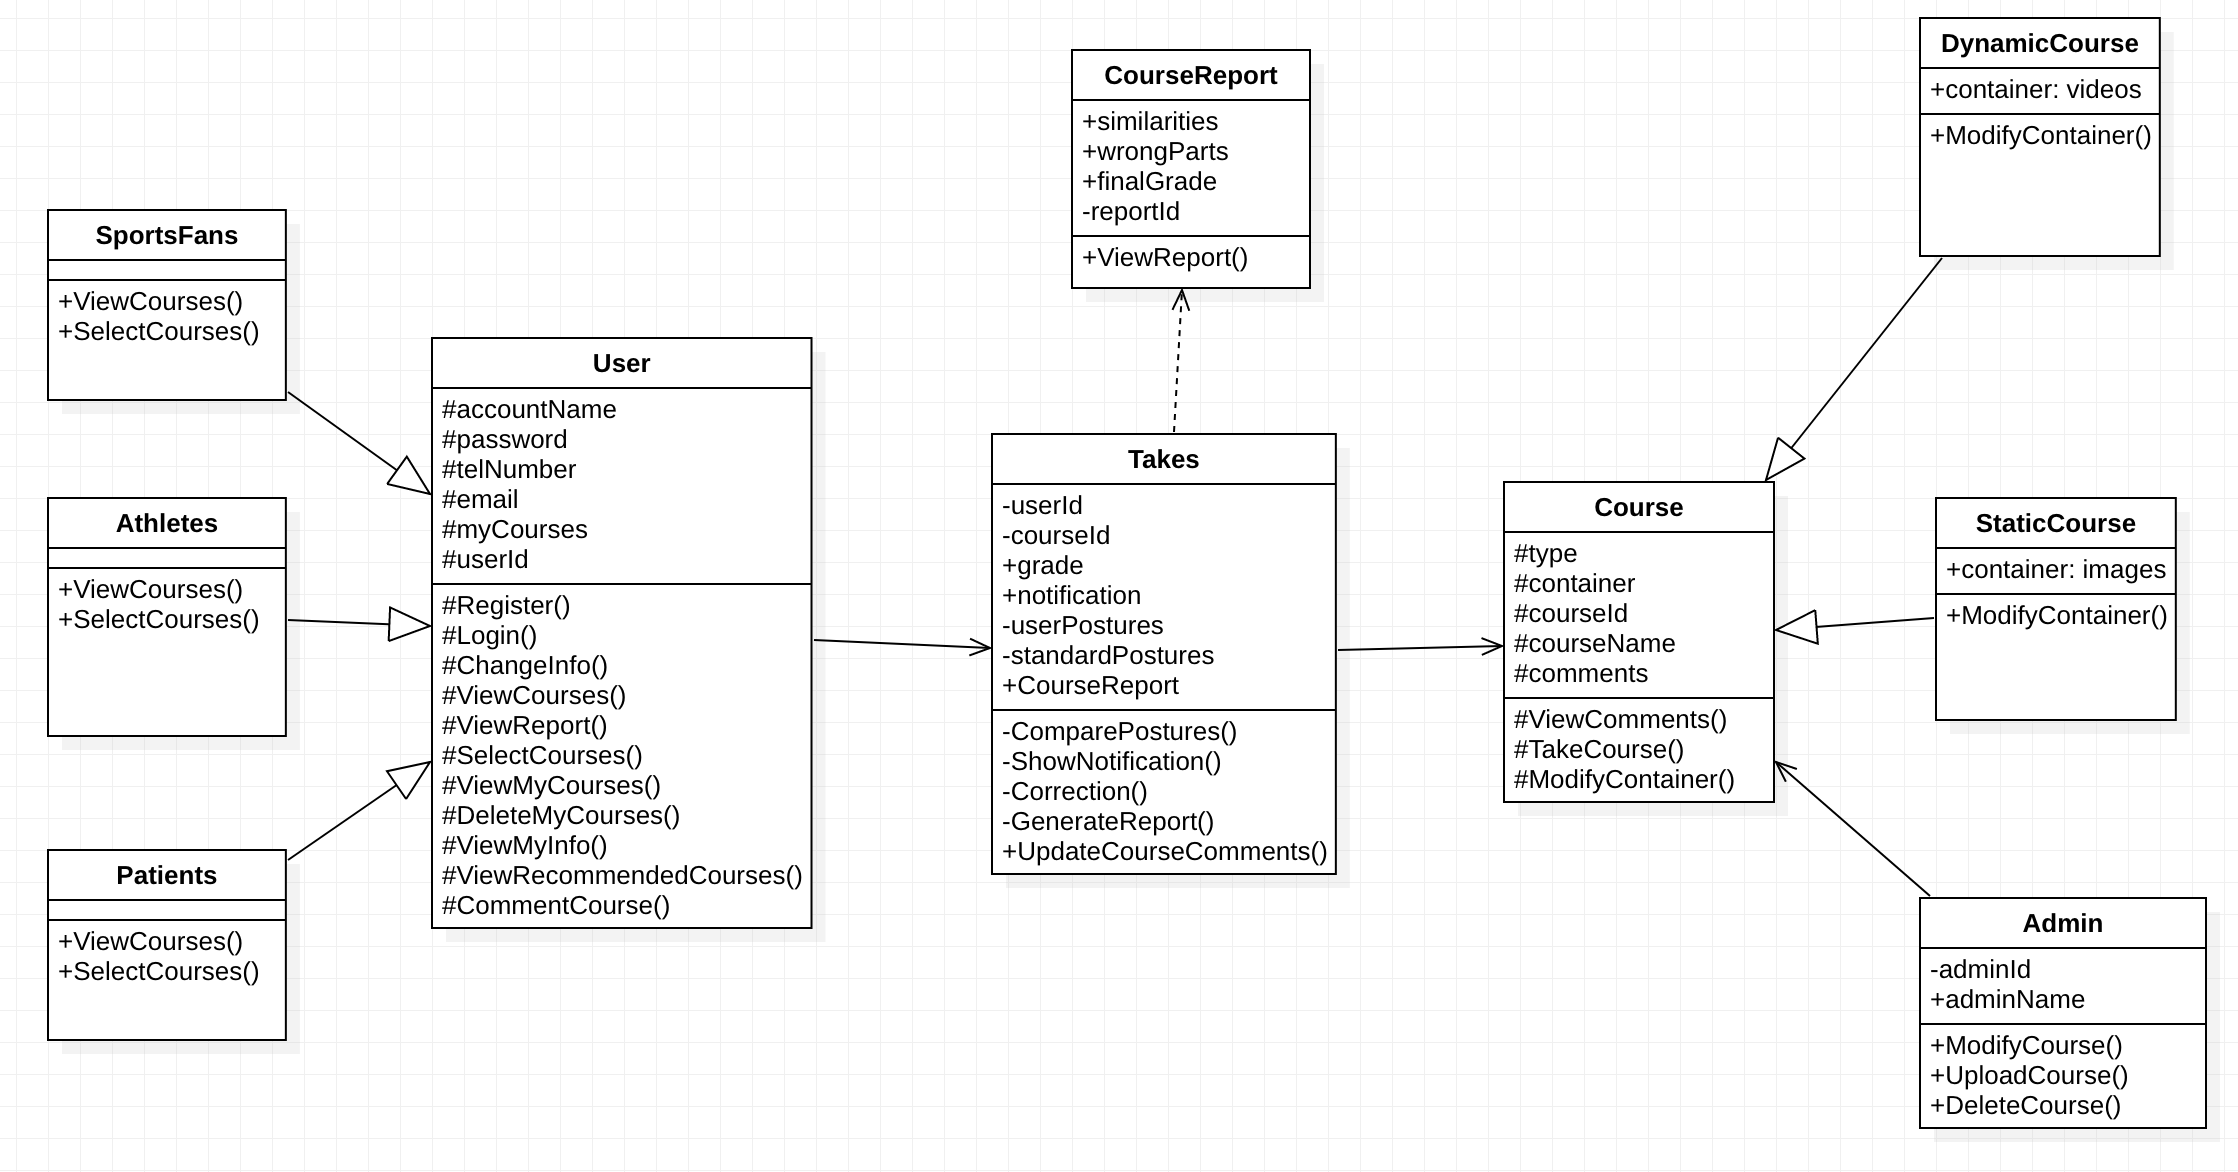
\includegraphics[width=1.1\textwidth]{figures/classDiagram.png}
\caption{Overview Class Diagram}
\label{fig:classdia}

\end{figure}
%\section{Hardware Interfaces}
%$<$Describe the logical and physical characteristics of each interface between 
%the software product and the hardware components of the system. This may include 
%the supported device types, the nature of the data and control interactions 
%between the software and the hardware, and communication protocols to be 
%used.$>$
\subsubsection{Attributes Description}
\begin{itemize}
	\item User = User's ID + Account Name + Password + Tel-Number + Email Address + User's Courses
	\item CourseReport = Report's ID + Postures' Similarities + User's Postures Wrong Parts + User's Final Grade
	\item Course = Course ID + Course Type + Videos/Images + Course Name + Comments
	\item Administrator = Administrator ID + Administrator Name
	\item Takes = User's ID + Corresponding Course ID + User's Final Grade + Notification + User's Postures + Standard Postures + Course Report
	\item SportsFans = User
	\item Athletes  = User
	\item DynamicCourse = Course with Videos
	\item StaticCourse = Course with Images
\end{itemize}
\subsubsection{Operations Description}
\begin{enumerate}
	\item Class User
	\begin{itemize}
		\item Register(): Apply for an account.
		\item Login(): Only after the user log in, he/she can use the functions of iSport.
		\item ChangeInfo(): To change the user's old information.
		\item ViewCourses(): View the courses, sports fans and athletes view exercise courses, patients view recover courses.
		\item ViewReport(): View the user's last training's report.
		\item SelectCourses(): Add courses to my courses. Sports fans and athletes add exercise courses, patients add recover courses.
		\item ViewMyCourses(): View the user's selected courses.
		\item DeleteMyCourses(): Remove courses from my courses.
		\item ViewMyInfo():  View the user's info.
		\item ViewRecommendedCourses(): View courses which is recommended by iSport system.
		\item CommentCourse(): Comment on a course.
	\end{itemize}
	\item Class Course
	\begin{itemize}
		\item ViewComments(): View this course's comments given by users.
		\item TakeCourse(): User decides to take this course.
		\item ModifyContainer(): Modify the videos or images of this course.
	\end{itemize}
	\item Class Takes
	\begin{itemize}
		\item ComparePostures(): Compare postures of the user and the standard images/videos.
		\item ShowNotification(): Show notification to the user when he/she takes courses.
		\item Correction(): Find what part of postures the user did wrong.
		\item GenerateReport(): Generate a report.
		\item UpdateCourseComment(): Update the course's comments.
	\end{itemize}
	\item Class SportsFans and Class Athletes
	\begin{itemize}
		\item ViewCourses(): Sports fans and athletes view exercise courses.
		\item SelectCourses(): Sports fans and athletes add exercise courses.
	\end{itemize}
	\item Class Patients
	\begin{itemize}
		\item ViewCourses(): Patients view recover courses.
		\item SelectCourses(): Patients add recover courses.
	\end{itemize}
	\item Class DynamicCourse
	\begin{itemize}
		\item ModifyContainer(): Modify the videos of this course.
	\end{itemize}
	\item Class StaticCourse
	\begin{itemize}
		\item ModifyContainer(): Modify the images of this course.
	\end{itemize}
	\item CourseReport
	\begin{itemize}
		\item ViewReport(): View this report.
	\end{itemize}
\end{enumerate}

\subsubsection{Class-Responsibility-Collaborator (CRC)}
\begin{enumerate}
	\item Class User
		\begin{figure}[H]
			\centering
			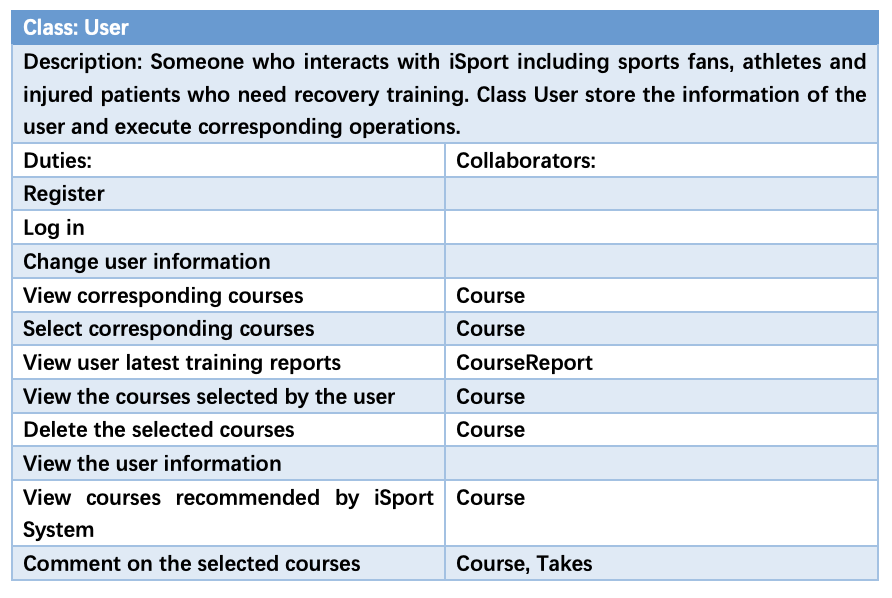
\includegraphics[width=1.1\textwidth]{figures/User.png}
			\caption{CRC Card for Class User}
			\label{fig:user}
		\end{figure}
	\item Class Course
		\begin{figure}[H]
			\centering
			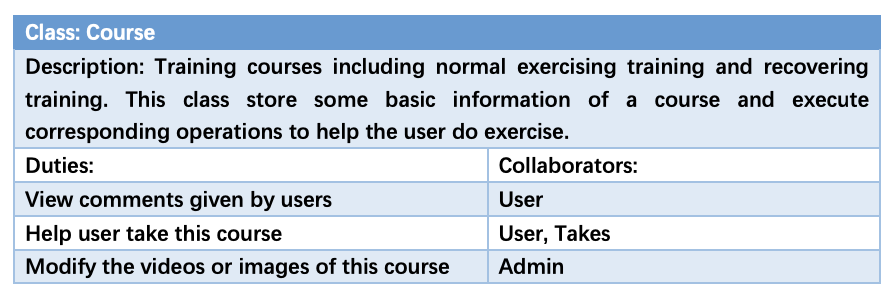
\includegraphics[width=1.1\textwidth]{figures/Course.png}
			\caption{CRC Card for Class User}
			\label{fig:course}
		\end{figure}
	\item Class Takes
		\begin{figure}[H]
			\centering
			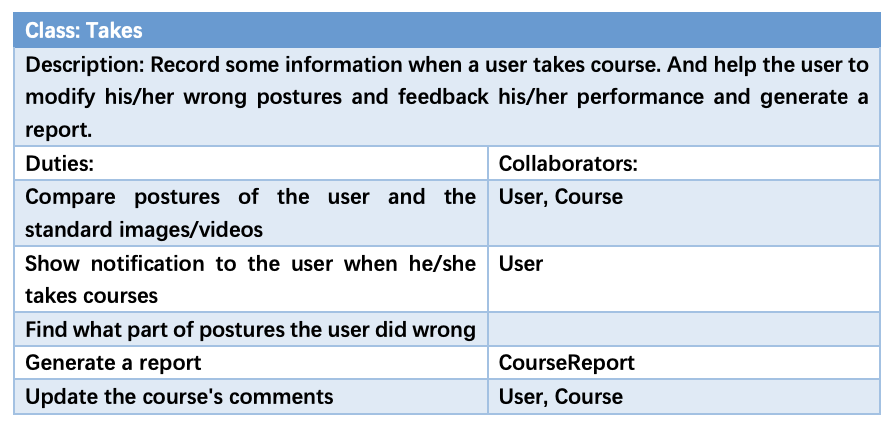
\includegraphics[width=1.1\textwidth]{figures/Takes.png}
			\caption{CRC Card for Class Takes}
			\label{fig:takes}
		\end{figure}
	\item Class CourseReport
		\begin{figure}[H]
			\centering
			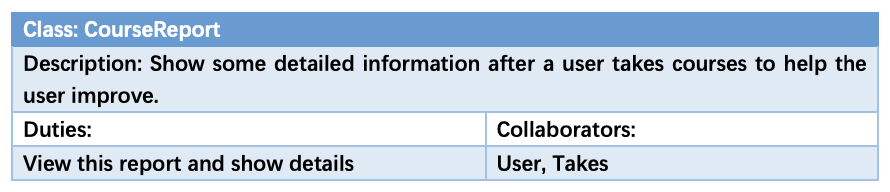
\includegraphics[width=1.1\textwidth]{figures/CourseReport.png}
			\caption{CRC Card for Class CourseReport}
			\label{fig:cr}
		\end{figure}
	\item Class Patients
		\begin{figure}[H]
			\centering
			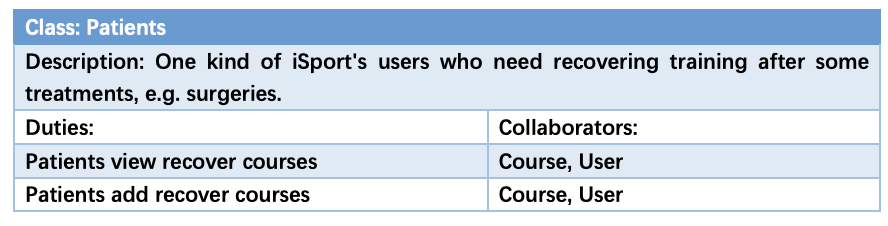
\includegraphics[width=1.1\textwidth]{figures/Patients.png}
			\caption{CRC Card for Class Patients}
			\label{fig:patients}
		\end{figure}
	\item Class Athletes and SportsFans
		\begin{figure}[H]
			\centering
			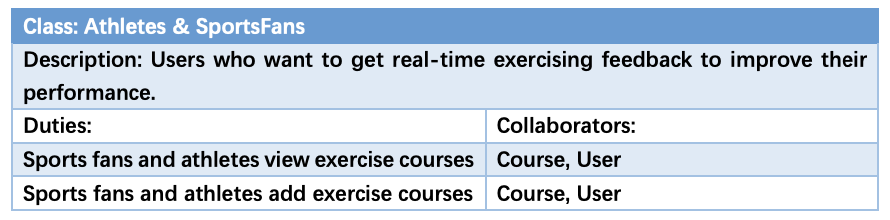
\includegraphics[width=1.1\textwidth]{figures/AthletesSports.png}
			\caption{CRC Card for Class Athletes and SportsFans}
			\label{fig:a_and_s}
		\end{figure}
	\item Class DynamicCourse
		\begin{figure}[H]
			\centering
			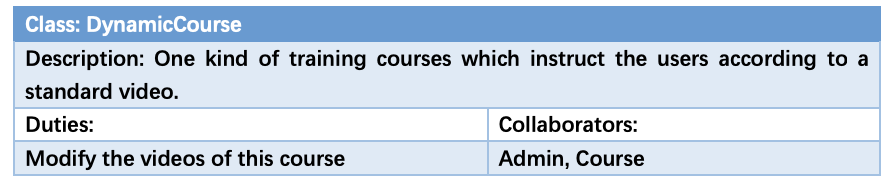
\includegraphics[width=1.1\textwidth]{figures/dynamic.png}
			\caption{CRC Card for Class DynamicCourse}
			\label{fig:dynamic}
		\end{figure}
	\item Class StaticCourse
		\begin{figure}[H]
			\centering
			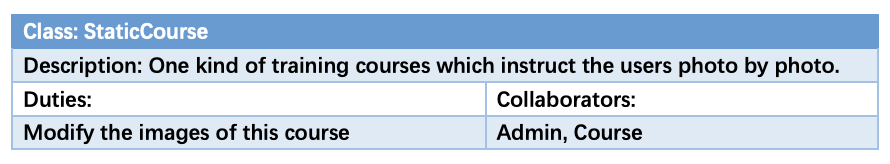
\includegraphics[width=1.1\textwidth]{figures/static.png}
			\caption{CRC Card for Class StaticCourse}
			\label{fig:static}
		\end{figure}
\end{enumerate}
\section{Behavior Requirements}

\subsubsection{Postural correction stateschart}

This stateschart describe the states transition during the process of postural correction.

\begin{figure}[H]
	\centering
	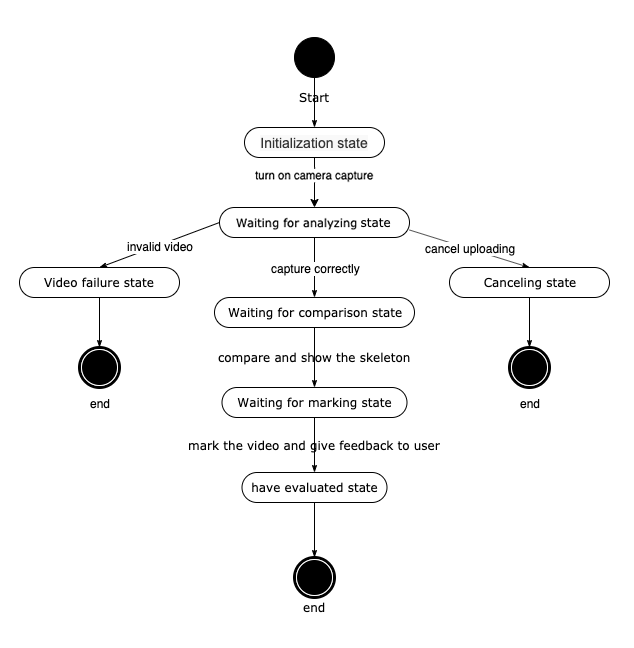
\includegraphics[width=1.0\textwidth]{figures/stateschart1.png}
	\caption{Postural correction statechart}
\end{figure}


\begin{center}
    \begin{tabular}{p{5cm}p{12cm}}
        \hline
	    Users & Desc\\
        \hline
	    Initialization state &  This state is the initialized posture correction process. User choose to turn on the camera capture, the state will shift to waiting for analyzing state \\
        \hline
	    Waiting for analyzing state & This state is waiting for analyzing. If the camera capture correctly, the state will shift to waiting for comparison state; if the video is invalid, the state will shift to video failure state; if the user cancel the uploading process, the state will shift to canceling state.\\
        \hline
        Waiting for comparison state & This state is waiting for comparison. The system will comparing and show the skeleton, and the state will shift to waiting for waiting for marking state\\
        \hline
        Waiting for marking state & This state is waiting for marking. After comparing, the system will mark user's posture, and the state will shift to have evaluated state\\
        \hline
        Video failure state & This state means the video is invalid, and the state will shift to terminate state\\
        \hline
        Canceling state & This state means the process was canceled by user, and the state will shift to terminate state\\
        \hline
        Have evaluated state & This state means the posture is finishing evaluation, and the state will shift to terminate state\\
        \hline
    \end{tabular}
\end{center}

\subsubsection{Course Evaluation statechart}

This stateschart describe the states transition during the process of course evaluation.

\begin{figure}[H]
	\centering
	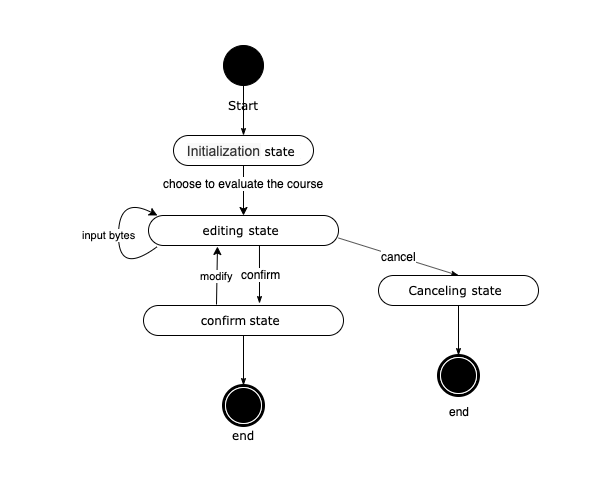
\includegraphics[width=1.0\textwidth]{figures/stateschart2.png}
	\caption{Course evaluation statechart}
\end{figure}


\begin{center}
    \begin{tabular}{p{5cm}p{12cm}}
        \hline
	    Users & Desc\\
        \hline
	    Initialization state &  This state is the initialized posture correction process. User choose to evaluate the course, the state will shift to editing state \\
        \hline
	    Editing state & This state is waiting for analyzing. If user is inputing bytes, the state will not change; if the user choose to confirm the evaluation, the state will shift to confirm state; if the user cancel the evaluation process, the state will shift to canceling state.\\
        \hline
        Confirm state & This state means the evaluation process is finished. If the user return to modify the comment, the state will shift to terminate state. In other condition, the state will shift to terminate state\\
        \hline
        Canceling state & This state means the process was canceled by user, and the state will shift to terminate state\\
        \hline
    \end{tabular}
\end{center}



\subsubsection{Posture information flow stateschart}

This stateschart describe the states transition of posture infomation flow

\begin{figure}[H]
	\centering
	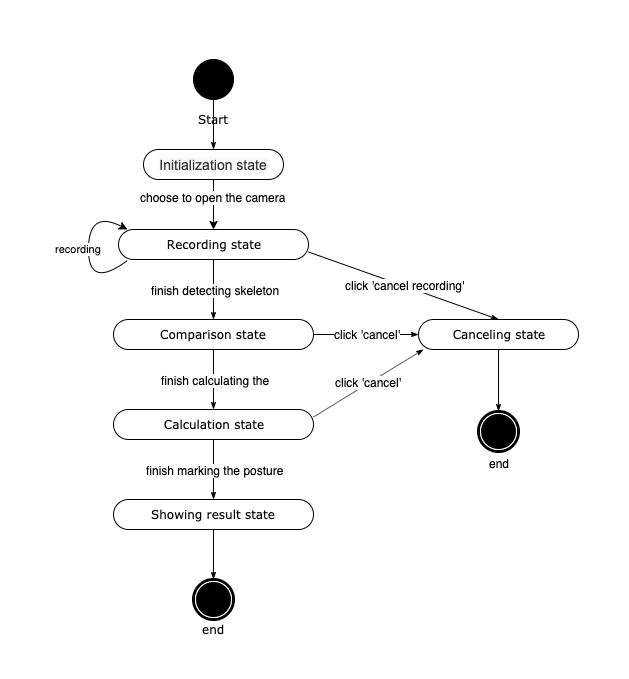
\includegraphics[width=1.0\textwidth]{figures/stateschart3.png}
	\caption{Posture information flow statechart}
\end{figure}


\begin{center}
    \begin{tabular}{p{5cm}p{12cm}}
        \hline
	    Users & Desc\\
        \hline
	    Initialization state &  This state is the initialized posture correction process. User choose to open the camera, the state will shift to waiting for recording state \\
        \hline
        Recording state & This state means the posture information is being recording. If the camera is recording video, the state will not change; if the skeleton data is detected, the state will shift to comparison state; if the user cancel the recording process, the state will shift to canceling state.\\
        \hline
        Comparison state & This state means the posture information is being comparing with the standard posture data. If the skeleton data is finished calculating, the state will shift to calculation state; if the user cancel the comparison process, the state will shift to canceling state.\\
        \hline
        Calculation state & This state means the posture information is being calculated after comparing with the standard posture data to get the mark of user's posture. If the skeleton data is finished marking the posture, the state will shift to showing result state; if the user cancel the calculation process, the state will shift to canceling state.\\
        \hline
        Canceling state & This state means the process was canceled by user, and the state will shift to terminate state\\
        \hline
        Show result state & This state means the posture information is finishing evaluation, the mark and suggestions will be show in user's interface, and the state will shift to terminate state\\
        \hline
    \end{tabular}
\end{center}




%\section{Software Interfaces}
%$<$Describe the connections between this product and other specific software 
%components (name and version), including databases, operating systems, tools, 
%libraries, and integrated commercial components. Identify the data items or 
%messages coming into the system and going out and describe the purpose of each.  
%Describe the services needed and the nature of communications. Refer to 
%documents that describe detailed application programming interface protocols.  
%Identify data that will be shared across software components. If the data 
%sharing mechanism must be implemented in a specific way (for example, use of a 
%global data area in a multitasking operating system), specify this as an 
%implementation constraint.$>$

%\section{Communications Interfaces}
%$<$Describe the requirements associated with any communications functions 
%required by this product, including e-mail, web browser, network server 
%communications protocols, electronic forms, and so on. Define any pertinent 
%message formatting. Identify any communication standards that will be used, such 
%as FTP or HTTP. Specify any communication security or encryption issues, data 
%transfer rates, and synchronization mechanisms.$>$


%\chapter{System Features}
%$<$This template illustrates organizing the functional requirements for the 
%product by system features, the major services provided by the product. You may 
%prefer to organize this section by use case, mode of operation, user class, 
%object class, functional hierarchy, or combinations of these, whatever makes the 
%most logical sense for your product.$>$
%
%\section{System Feature 1}
%$<$Don’t really say “System Feature 1.” State the feature name in just a few 
%words.$>$
%
%\subsection{Description and Priority}
%$<$Provide a short description of the feature and indicate whether it is of 
%High, Medium, or Low priority. You could also include specific priority 
%component ratings, such as benefit, penalty, cost, and risk (each rated on a 
%relative scale from a low of 1 to a high of 9).$>$
%
%\subsection{Stimulus/Response Sequences}
%$<$List the sequences of user actions and system responses that stimulate the 
%behavior defined for this feature. These will correspond to the dialog elements 
%associated with use cases.$>$
%
%\subsection{Functional Requirements}
%$<$Itemize the detailed functional requirements associated with this feature.  
%These are the software capabilities that must be present in order for the user 
%to carry out the services provided by the feature, or to execute the use case.  
%Include how the product should respond to anticipated error conditions or 
%invalid inputs. Requirements should be concise, complete, unambiguous, 
%verifiable, and necessary. Use “TBD” as a placeholder to indicate when necessary 
%information is not yet available.$>$
%
%$<$Each requirement should be uniquely identified with a sequence number or a 
%meaningful tag of some kind.$>$
%
%REQ-1:	REQ-2:
%
%\section{System Feature 2 (and so on)}


\chapter{Other Nonfunctional Requirements}
\label{Other Nonfunctional Requirements}
\section{Performance Requirements}
\subsection{Precision}
\subsubsection{Input precision}
Phone number: 11 digits, will convert to string in database. \\
Email: numbers or letters, regex pattern: /\^([A-Za-z0-9\_$\backslash$-$\backslash$.])+$\backslash$.([A-Za-z]\{2,4\})\$/. \\

\subsection{Time speciality requirement}
\subsubsection{Response time}
\begin{itemize}
    \item loading webpages time should be less than 1 second;
    \item operating webpage widget should be less than 0.5 second;
    \item when network is in good condition, the information loading time should be less than 0.5 second;
    \item when network is in good condition, user comment and report should be up to date in 2 seconds after user add a new one.
    \item adopt message middleware, update should be async, do not affect the main process UI response.
    \item all pages updating should be async, and the priority of character loading is larger than photo's, time of updating character should be less than 0.1 second, time of updating photos should be less than 0.2 second.
    \item all the page updating time should be less than 1 second.
\end{itemize}

\subsection{Input and output requirement}
\subsubsection{User register input}
data name: user register input data
implication: for usr registration, including user name and password
data type: string
constraint: consist of English letters and numbers, no special characters allowed. The length of username is between 6 and 12, password is between 6 and 18.
\subsubsection{User comments input}
data name: user comments input data
implication: for user comments 
data type: string
constraint: length of comments should be at least 10 words and less than 500 words.

\section{Safety and Security Requirements}
The frontend and backend should both check the input data to ensure the user input won't cause a system crash.\\
Some sensitive data, including phone numbers and email address is store in database, once divulged, the user may be affected by harass message. The database authorization should be granted with caution.\\ 
Some days the system should be deployed in disturbed system, maintaining consistency by consensus algorithm, avoiding data safety, minimize the danger of dropping data caused by crash.\\

\section{Software Quality Attributes}
\subsection{Flexibility Requirement}
We use iterative development, in a week, for a development cycle, check every three days to discuss the progress of the development, after the end of each iteration to joint test of existing functions, to ensure that when the former system can run normally after discussing the development of the next increment details and concrete tasks, we carried out in accordance with the system module division of labor, each member is responsible for the view, model, control device and block chain one of four modules or some modules of all the work, each mold piece in have different emphases, members based on their ability to select the corresponding module development,
Docking test will be conducted between modules after completion of development\\
The development mode of test-driven development is adopted. After the development task is determined, the corresponding unit test is written first. The code written during functional development needs to pass the unit test written at the beginning to ensure the writing efficiency and quality of the code.\\
Git is adopted for project management, and corresponding records are kept for each function update and version iteration. If the plan needs to be changed or improved, the most appropriate version can be selected to continue development based on the original development.
This approach reduces the additional development effort due to planned changes and allows us to be more flexible with the changes we encounter during development.\\
We will adopt a backward compatible development plan in the development process, that is, our system can be well adapted to the new environment in the future, and the client supports a variety of system adaptations, and can work well on different types of devices.\\
The relevant interface information of the system is stored in the database. If the software interface of the foreign department changes during the system operation, the content in the database can be modified to adapt to the change\\

\subsection{Reliability Requirement}
The entire system will be distributed in the form of a database so that each participating node can get a copy of the complete database.
Unless more than 51\% of nodes in the entire system can be controlled at the same time, changes to the database on a single node are not valid and cannot affect the data content on other nodes.

\subsection{Usability Requirement}
\begin{itemize}
    \item The unified interface style and friendly user interaction design make it more convenient for users to acquire
The information you want.
    \item Reduce the user's learning cost as far as possible, convenient operation, reasonable operation process, the completion of the operation when the unified standard prompt information.
    \item Support no computer use experience, less computer use experience and have more computer use experience users can easily use the system
    \item The system has a certain fault-tolerant and anti-interference ability, in the non-hardware fault or non-communication fault, the system can ensure the normal operation, and there are enough prompt information to help users effectively and correctly complete the task.
    \item The system has some flexibility, can prompt the user how to operate
    \item The system is universal, easy to learn and practical
    \item The site features fewer features and fewer redundant and annoying features.
\end{itemize}

\subsection{Maintainability Requirement}
\begin{itemize}
    \item Maintainability is the ability to modify problems or defects in existing system functionality without affecting the rest of the system.
When developers create and design system architectures, they must consider the following elements in order to improve system maintainability: low-coupling, high-in-aggregate systems.
    \item This system will adopt strict software engineering specification to develop, and adopt good design mode to ensure the low coupling and high cohesion between the modules.
    \item All the code of the system will be detailed comments, for all the code of the system, we will generate detailed technical documentation.
For the system development process may appear error, we will document the way a detailed list of error and corresponding error message.
    \item Relevant documentation should be clear, complete and consistent
    \item At the same time, it should have good function, data extensibility and adaptability to the environment
\end{itemize}

\subsection{Expandability Requirement}
After the completion of the system, no major changes should be made to the existing system or affect the whole system
In this way, it is convenient to add corresponding functions according to the needs of users in the later maintenance process without affecting the normal operation of other function modules of the system.
In addition, all documentation should be detailed and complete so that other recipients or new developers can quickly learn about the system and properly update and enhance it.

\subsection{Stability Requirement}
The website can normally complete all functional requirements, and ensure that the server runs for a long time without obstacles.
Fault repair time is generally controlled within 3 hours, unless there is a vicious attack, virus damage, insufficient system resources, hardware failure, operating system crash network interruption, do not allow memory leak.
The system is required to be able to withstand the warning storm and the impact of the large amount of data, not memory overflow and other phenomena.

\subsection{Operational Environment Convertibility Requirements}
This web page can be self-adapted to normal operation on the mobile phone.


\chapter{Other Requirements}
\label{Other Requirements}
$<$Define any other requirements not covered elsewhere in the SRS. This might 
include database requirements, internationalization requirements, legal 
requirements, reuse objectives for the project, and so on. Add any new sections 
that are pertinent to the project.$>$

\section{Data Dictionary Requirements}
$<$ $>$

%\section{Appendix A: Glossary}
%%see https://en.wikibooks.org/wiki/LaTeX/Glossary
%$<$Define all the terms necessary to properly interpret the SRS, including 
%acronyms and abbreviations. You may wish to build a separate glossary that spans 
%multiple projects or the entire organization, and just include terms specific to 
%a single project in each SRS.$>$

\section{Appendix A: Analysis Models}
$<$Optionally, include any pertinent analysis models, such as data flow 
diagrams, class diagrams, state-transition diagrams, or entity-relationship 
diagrams.$>$

\section{Appendix B: To Be Determined List}
$<$Collect a numbered list of the TBD (to be determined) references that remain 
in the SRS so they can be tracked to closure.$>$

\end{document}
